\documentclass[aps,prb,10pt,showpacs,superscriptaddress,twocolumn,notitlepage]{revtex4-1}
\usepackage{amsmath}

\usepackage{graphicx}
\graphicspath{{figures/}{./}}

\usepackage[colorlinks=true, linkcolor=blue, citecolor=red]{hyperref}

\pacs{71.35.Cc, 73.20.Mf, 71.15.Mb, 71.20.Mq, 71.10.-w}

\begin{document}

\title{Plasmon dispersion in Graphite: A comparison of current \emph{ab initio}
methods}
\author{Sean M. Anderson}\email{sma@cio.mx}
    \affiliation{Centro de Investigaciones en \'Optica, 
                Le\'on, Guanajuato, M\'exico}
\author{Bernardo S. Mendoza}%\email{bms@cio.mx}
    \affiliation{Centro de Investigaciones en \'Optica, 
                Le\'on, Guanajuato, M\'exico}
\author{Giorgia Fugallo}%\email{giorgia.fugallo@univ-nantes.fr}
    \affiliation{Laboratoire des Solides Irradi\'es, \'Ecole Polytechnique, 
    CNRS, CEA, Université Paris-Saclay, F-91128 Palaiseau, France }
    \affiliation{European Theoretical Spectroscopy Facility (ETSF)}
\author{Francesco Sottile}%\email{francesco.sottile@polytechnique.fr}
    \affiliation{Laboratoire des Solides Irradi\'es, \'Ecole Polytechnique, 
    CNRS, CEA, Université Paris-Saclay, F-91128 Palaiseau, France }
    \affiliation{European Theoretical Spectroscopy Facility (ETSF)}
\date{\today}

\begin{abstract}
We perform a systematic study of the macroscopic dielectric function and EEL
spectra for graphite over an energy range that encompasses both the $\pi$ and
$\pi + \sigma$ plasmons. We obtain the dispersion behavior of both of these
plasmons, as a function of the momentum transfer $q$ for two non-equivalent
paths that traverse the first four Brillouin zones. We carry out these
calculations within both time-dependent density functional theory (with two
exchange-correlation functionals) and the Bethe-Salpeter equation. Additionally,
we explore the effects of using the complete excitonic Hamiltonian (with all e-h
pairs and antipairs), and within the Tamm-Dancoff approximation (neglecting
antipairs). We accurately discern which peaks derive from plasmonic behavior or
from interband transitions and accurately compare these outcomes against several
experiments that span almost five decades. Our results present clear trends that
follow the physical origins of the observed peaks. We carry out this study over
large ranges of both energy and momentum transfer in order to better evaluate
the different theoretical methods compared to experiment, and predict the
plasmonic behavior beyond available experimental data.
\end{abstract}

\maketitle

%%%%%%%%%%%%%%%%%%%%%%%%%%%%%%%%%%%%%%%%%%%%%%%%%%%%%%%%%%%%%%%%%%%%%%%%%%%%%%%%
%%%%%%%%%%%%%%%%%%%%%%%%%%%%%%%%%%%%%%%%%%%%%%%%%%%%%%%%%%%%%%%%%%%%%%%%%%%%%%%%

\section{Introduction}\label{sec:intro}

The study of the optical spectra of solids yields important insight into the
underlying electronic and structural properties of a material. When an incident
photon is absorbed by a material, the system is energetically excited from its
ground to an excited state, forming an electron-hole pair or exciton, a
localized quantum of neutral electron-hole (e-h) pairs bound by the Coulomb
attraction. From a theoretical standpoint, \emph{ab initio} calculations are
essential tools for elucidating these excited-state electronic properties of
solids, surfaces, and nanostructures. Ground state properties can be calculated
accurately using density functional theory (DFT) \cite{hohenbergPR64, kohnPR65},
but the aforementioned electronic excitations necessitate further theoretical
developments. Time-dependent density functional theory (TDDFT) \cite{rungePRL84}
is a natural extension of DFT, and is able to successfully describe spectra like
electron energy loss spectrosopy (EELS) or Inelastic X-ray scattering of simple
semiconductors, as well as the photo-absorption cross-section of simple
molecules. However, while the use of the local density approximation (LDA) in
DFT yields qualitative (and more often than not, quantitative) agreement with
experiment for the ground state properties of many materials,the same cannot be
said for using the adiabatic LDA (ALDA) functional \cite{rungePRL84} in TDDFT
(the TDDFT equivalent of DFT-LDA). This functional does not consistently improve
the calculated optical spectra of solids with respect to the common random phase
approximation (RPA) where the exchange-correlation functional, the main
ingredient of TDDFT, is neglected. It is in fact well known \cite{onidaRMP02}
that today functionals and approximattions to TDDFT are not well-suited for
accurately calculating the absorption spectra of most solids
\cite{gavrilenkoPRB97, onidaRMP02}, where excitonic behavior predominates.

Thus, the behavior of complex electronic excitations can only be accurately
described by making use of many-body perturbation theory (MBPT)
\cite{fetterbook72}. In particular, using Hedin's GW approximation
\cite{hedinPR65} followed by solving the Bethe-Salpeter equation (BSE)
\cite{salpeterPR51, abrikosovbook65, shamPR66, hankePRB80, onidaRMP02} allows
for the accurate calculation of the optical properties of many physical systems,
within a completely \emph{ab initio} framework \cite{shirleyPRL93,
albrechtPRB97, benedictPRL98, benedictPRB99, benedictPRB03, palummoJPCM04,
sittPRA07, ramosPRB08, roccaJCP10, garciaJCP11, gruningCMS11, gattiPRB13}.

In general, absorption and scattering spectroscopies (that concern neutral
excitations), are very well described by the BSE \cite{onidaPRL95, albrechtPRL98,
benedictPRB98, rohlfingPRL98b, onidaRMP02}. Within this GW/BSE approach,
excitons are described as a combination of e-h pairs of a noninteracting system;
we can convert the problem to an effective eigenvalue problem in the e-h basis.
However, nanoscale materials involve a huge number of e-h pairs, which makes
solving the BSE extremely costly from a computational standpoint. The
Tamm-Dancoff approximation (TDA) \cite{fetterbook72} is an approximation that
only considers positive energy e-h pairs, effectively neglecting the interaction
between e-h pairs at positive and negative (antipairs) energies. The
non-Hermitian BS problem is thus reduced to a Hermitian problem that can be
solved with efficient and stable iterative methods. The Haydock recursion scheme
\cite{haydockJPC72, haydockCPC80, roccaJCP08} is one of the most efficient and
computationally inexpensive iterative methods used for dealing with the
Hamiltonian. Thanks to this reduction in the computational complexity, the TDA
has been applied to a variety of systems \cite{lopezPRL06, arnaudPRL06,
wirtzPRL06}.

Excitations from plasmons, collective oscillations of the electronic density
that induce a macroscopic polarization, can also feature very prominently in the
measured EEL spectra for some materials. These oscillations involve the creation
of e-h antipairs; thus, these plasmonic features are inherently ill-described by
the TDA \cite{zimmermannPSSB70, caliebePRL00, olevanoPRL01, gruningNL09}.
Accurately describing both plasmonic and excitonic features is essential if we
wish to accurately characterize and analyze the system; therefore, we require a
suitable test case in order to carry out a complete study of these theoretical
methods. Optimally, this reference material will display plasmonic behavior, be
theoretically and experimentally well-characterized, and have continued
relevance in current research. We consider that bulk graphite meets these
requirements and can make for a very effective benchmark. Early work revealed
accurate band structure calculations \cite{bassaniINCB1967, painterPRB70}, that
continue to be experimentally studied by very precise photoemission and ARPES
experiments \cite{gruneisPRL08, matsuiPRB18}. A great variety of EELS
\cite{taftPR65, zeppenfeldZP71, venghausPSSB1974, buchnerPSSB77,
marinopoulosPRL02, krambergerPRL08} and absorption \cite{linPRB97,
krambergerPRL08, trevisanuttoPRB10} measurements have been carried out with
relevant theoretical developments, including detailed analysis of the low-energy
($\pi$) and high-energy ($\pi + \sigma$) plasmons. Concerning the actual plasmon
dispersion, there is very recent work \cite{kinyanjuiEPL12, liouPRB15} featuring
very high-resolution EELS measurements for a variety of values of momentum
transfer. Lastly, graphite continues to be of relevance as the precursor of
graphene, which presents its own unique spectroscopic characteristics
\cite{yangPRL09, tegenkampJPCM11, politanoNS14, liouPRB15, bulushevaIJQC16,
liPRB17}, many of which can be explained through its relationship with graphite.

In this paper, we perform a systematic study of the macroscopic dielectric
function and EEL spectra for graphite, in order to elucidate the $\pi$ and $\pi
+ \sigma$ plasmon dispersion behavior as a function of the momentum transfer $q$
for two non-equivalent paths that encompass the first four Brillouin zones. We
carry out these calculations within both TDDFT (with two exchange-correlation
functionals) and the BSE; additionally, we explore the effects of using the
complete excitonic Hamiltonian (with all e-h pairs and antipairs), and within
the TDA (neglecting antipairs). The resulting spectra are consistent with
previous results featured in the literature, and we can accurately discern which
peaks derive from plasmonic behavior or from interband transitions. However, as
each method considers very different approximations, the peak positions and
intensity change substantially. We accurately study these characteristics and
compare them against several experiments taken in different decades and by
different groups. Our calculated spectra present clear trends that follow the
physical origins of the observed peaks. Given the large energy range that we
consider in this work (from 0 to 45 eV), the large momentum transfer values (up
to $q = 3.22$ \r{A}$^{-1}$), and the comparison of several methods with various
experiments, we consider this to be a thorough benchmark for future reference.

This paper is organized as follows. In Sec. \ref{sec:theory}, we present the
theoretical framework that describes the aforementioned methods. In Sec.
\ref{sec:results}, we present our results for the $q$-dependent plasmon
dispersion over two separate, non-equivalent paths in the Brillouin zone, and
show several detailed comparisons with experiment. We list our conclusions and
final remarks in Sec. \ref{sec:conclusions}. Lastly, Appx. \ref{sec:bench}
includes real-world computational performance benchmarks for each of the
calculations included in this paper.

%%%%%%%%%%%%%%%%%%%%%%%%%%%%%%%%%%%%%%%%%%%%%%%%%%%%%%%%%%%%%%%%%%%%%%%%%%%%%%%%
%%%%%%%%%%%%%%%%%%%%%%%%%%%%%%%%%%%%%%%%%%%%%%%%%%%%%%%%%%%%%%%%%%%%%%%%%%%%%%%%

\section{Theory}\label{sec:theory}

In order to better explain the differences between the TDDFT and BSE frameworks,
we will describe them in the same formalism for clarity and ease of
interpretation. The key quantity measured in absorption and EELS is the
macroscopic dielectric function, $\epsilon_{\mathrm{M}}$; specifically,
$\mathrm{Im}\,\epsilon_{\mathrm{M}}$ is measured in absorption experiments,
while $-\mathrm{Im}\,(1/\epsilon_{\mathrm{M}})$ is measured in EELS. The
macroscopic dielectric function is connected to the inverse dielectric function
$\epsilon^{-1}$ as
\begin{equation}
\epsilon_{\mathrm{M}}(\omega)\equiv
\lim_{\mathbf{q}\to 0}
\frac{1}{[\epsilon^{-1}(\mathbf{q},\omega)]_{\mathbf{G = G^{\prime}} = 0}},
\end{equation}
where $\mathbf{G}$ and $\mathbf{G^{\prime}}$ are reciprocal lattice vectors. We
can express $\epsilon^{-1}$ for both TDDFT and the BSE as a Dyson-like equation,
\begin{equation}\label{eq:dyson}
D = D^{(0)} + D^{(0)}KD.
\end{equation}
For TDDFT, $D$ is the two-point polarizability $\chi$, from which we can obtain
the inverse dielectric function $\epsilon^{-1} = 1 - v\chi$ ($v$ is the Coulomb
potential); for the BSE, $D$ is the two-particle correlation function $L$ which
yields $\chi$ by contracting two of its four indices,
\begin{equation}\label{eq:ki}
\chi(1, 2) = L(1, 1^{+}, 2, 2^{+}),
\end{equation}
where $(1)$ is shorthand notation for specific position, time, and spin states.

The two theories can be recast in the same equation, but this similarity in form
hides some key differences \cite{luciabook, sottilePRL03}:
\begin{itemize}
\item TDDFT leads to two point equations for describing the propagation of the
density; BSE describes the propagation of an electron (e) and a hole (h), and
thus leads to four point equations (as evident from  Eq. \ref{eq:ki}).
\item In TDDFT, $D^{(0)}$ is the independent-particle response function
$\chi^{(0)}$ constructed with the Kohn Sham (KS) orbitals and eigenvalues; in
the BSE formalism, $D^{(0)}$ is the independent quasiparticle response $L^{(0)}$
constructed using quasiparticle eigenvalues and eigenfunctions (obtained, for
example, via a GW calculation as done in this work).
\item In TDDFT, the kernel $K = v + f_{xc}$, where $f_{xc}$ is the functional
derivative with respect to the density of the exchange-correlation potential
$v_{xc}$, and so $f_{xc} = \delta v_{xc}/\delta\rho$. For the BSE, $K = v - W$
with $W$ the screened version of the bare Coulomb interaction $v$.
\end{itemize}
Regarding this last point, different approximations are possible for $v_{xc}$
and thus $f_{xc}$. In this work, we will compare the adiabatic local density
approximation (ALDA) where the exchange-correlation potential is taken in the
LDA,
\begin{equation}
f^{\mathrm{ALDA}}_{xc} = \delta v^{\mathrm{LDA}}_{xc}/\delta\rho,
\end{equation} 
and the random phase approximation (RPA) where
\begin{equation}
f^{\mathrm{RPA}}_{xc} = 0.
\end{equation}
In the case of the BSE, the screening term $W$ is commonly taken in a static
version calculated at the RPA level \cite{onidaRMP02, luciabook}. While $v$
enters in the kernel $K$ as a repulsive e-h exchange interaction and is
responsible for the local-field effects, the second term in both theories
($f_{xc}$ or $-W$) describes the attractive interaction which is the origin of
the excitonic effects, including the formation of bound excitons.
 
In order to obtain a spectral representation of $D$, it is useful to reformulate
the Dyson-like Eq. \ref{eq:dyson} as an eigenvalue problem \cite{rohlfingPRB00,
onidaRMP02} by introducing an effective two-particle excitonic Hamiltonian,
$H_{\mathrm{exc}}$, thus obtaining an eigenvalue problem,
\begin{equation}
H_{\mathrm{exc}}(\mathbf{q_{r}}) A_{\lambda}(\mathbf{q_{r}}) =
E_{\lambda}(\mathbf{q_{r}})      A_{\lambda}(\mathbf{q_{r}}).
\end{equation}
The excitonic Hamiltonian is written in a basis of electron-hole transitions
($n_{1}k_{1} \rightarrow n_{2}k_{2}$). These transitions can be classified as
resonant  transitions, $(v, k - q_{r}) \rightarrow (c, k)$, or anti-resonant
transitions, $(c, k) \rightarrow (v, k + q_{r})$, depending on if the band index
$n$ is associated with an occupied valence (v) band or an unoccupied conduction
(c) band. Lastly, $q_{r}$ is a momentum transfer belonging to the first
Brillouin zone \cite{gattiPRB13}. The excitonic hamiltonian has a block matrix
form \cite{gattiPRB13, albrechtPRL98, olevanoPRL01, gruningCMS11},
\begin{equation}
H_{\mathrm{exc}} =
\left(
\begin{array}{c c}
R       & C^{R,A} \\
C^{A,R} & A       \\
\end{array}
\right).
\end{equation}
When working in the long-wavelength limit ($q_{r} \rightarrow 0$), $A = -R^{*}$
and $C^{A,R} = -\left[C^{R,A}\right]^{*}$. The diagonal $A$ and $R$ blocks are
Hermitian, while the coupling $C$ blocks are symmetric. When dealing with a
generic momentum transfer $q_{r} \neq 0$ then $A \neq -R^{*}$ and the coupling
terms are no longer symmetric, effectively doubling the computational cost of
evaluating $H_{\mathrm{exc}}$.

By taking advantage of the fact that the off-diagonal terms are typically
significantly smaller than the resonant terms, it is possible to reduce the
computational cost by using the Tamn-Dancoff approximation (TDA)
\cite{fetterbook72} by setting the off-diagonal coupling terms $C$ to zero. In
other words, the interaction between e-h pairs at positive and negative
(antipairs) energies is neglected, and only one e-h pair is assumed to propagate
in any time interval. Considering the different nature and locality of excitons
and plasmons, it is clear that the TDA is more unreliable for describing
plasmons, where the density oscillations involve the excitation of large numbers
of e-h antipairs. Nevertheless, due to the success obtained in describing the
optical absorption of solids and thanks to the remarkable numerical advantages,
the TDA has been applied to many different systems \cite{luciabook}. Under the
TDA the Hamiltonian becomes a Hermitian operator, enabling the use of efficient
iterative schemes for solving the BSE such as the Haydock recursion method
\cite{haydockJPC72, haydockCPC80, benedictPRB99, roccaJCP08, gruningCMS11,
ljungbergPRB15}.
 
Regardless of the framework (TDDFT or BSE) or the method used for diagonalizing
the excitonic Hamiltonian, it is possible to obtain the macroscopic dielectric
function from the eigenvalues ($E_{\lambda}$) and eigenstates ($A_{\lambda}$);
\cite{onidaRMP02} this is then used to calculate the theoretical spectra that
can be directly compared with experimental data. Note that for large momentum
transfer,
\begin{equation}\label{eq:eels}
\begin{split}
-\mathrm{Im}\,\epsilon_{\mathrm{M}}(\mathbf{q}, \omega)
&= \frac{\mathrm{Im}\,\epsilon_{\mathrm{M}}(\mathbf{q}, \omega)}
        {[\mathrm{Re}\,\epsilon_{\mathrm{M}}(\mathbf{q}, \omega)]^{2} +
         [\mathrm{Im}\,\epsilon_{\mathrm{M}}(\mathbf{q}, \omega)]^{2}}\\
&\approx \mathrm{Im}\,\epsilon_{\mathrm{M}}(\mathbf{q}, \omega),
\end{split}
\end{equation}
since $\mathrm{Re}\,\epsilon_{\mathrm{M}}(\mathbf{q}, \omega) \rightarrow 1$,
and $\mathrm{Im}\,\epsilon_{\mathrm{M}}(\mathbf{q}, \omega)$ is very small
\cite{gattiPRB13}. Thus, the EEL spectra will increasingly mimic the absorption
spectra for large values of $q$. A plasmon excitation is identified as the point
where $\mathrm{Re}\,\epsilon_{\mathrm{M}} = 0$ (crossing from negative to
positive), and $\mathrm{Im}\,\epsilon_{\mathrm{M}}$ is nearly zero. For
convenience, we will refer to this as the plasmon criterion
\cite{jonesbookv11973}; therefore, peaks in the EEL spectra that meet this
condition will naturally be understood to be plasmon excitations.

Table \ref{tab:names} enumerates the labels that we will use for the remainder
of this work, and the particular method described by each label.

\begin{table}[b]
\caption{Naming scheme employed for the calculations featured in this work.}
\label{tab:names}
\begin{ruledtabular}
\begin{tabular}{ r l c c c }
\multicolumn{2}{c}{Label}  & Type   & Hamiltonian  & $f_{xc}$ \\
\hline
BSE  & CP/TD & MBPT  & Full/Tamm-Dancoff & -- \\
ALDA & CP/TD & TDDFT & Full/Tamm-Dancoff & $\delta v^{\mathrm{LDA}}_{xc}/\delta\rho$ \\
RPA  & CP/TD & TDDFT & Full/Tamm-Dancoff & $0$
\end{tabular}
\end{ruledtabular}
\end{table}


%%%%%%%%%%%%%%%%%%%%%%%%%%%%%%%%%%%%%%%%%%%%%%%%%%%%%%%%%%%%%%%%%%%%%%%%%%%%%%%%
%%%%%%%%%%%%%%%%%%%%%%%%%%%%%%%%%%%%%%%%%%%%%%%%%%%%%%%%%%%%%%%%%%%%%%%%%%%%%%%%

\section{Computational Details}\label{sec:comp}

The electronic ground state and band structure of bulk graphite was calculated
using DFT-LDA \cite{hohenbergPR64, kohnPR65}, using norm-conserving
Troulliers-Martins pseudopotentials \cite{troullierPRB91} using the plane-wave
basis method implemented within the ABINIT\cite{gonzeCPS09, abinit} code. Our
calculated DFT band structure is identical to previously reported results
\cite{marinopoulosPRB04}. We constructed the graphite structure using lattice
constants $a = 2.45$ \r{A} and $c = 6.69$ \r{A}, obtained from structural
optimization studies. The ground state energy was calculated using a
11$\times$11$\times$4 Monkhorst-Pack grid of \textbf{k}-points, with an energy
cutoff of 20 Ha.

We then selected two separate \textbf{k}-point grids for carrying out our study
of plasmon dispersion over different momentum values, $q$. These momentum
vectors follow two in-plane paths along the Brillouin zones; first, from
$\Gamma$ to the M point of the fourth zone (M$_{4}$), and second, from $\Gamma$
to the K point of the fourth zone (K$_{4}$). Both paths pass through various
points of symmetry; see Fig. \ref{fig:brillouin} for a graphical representation.
The selected $\Gamma$-centered 14$\times$14$\times$2 (392 \textbf{k}-points) and
12$\times$12$\times$2 (288 \textbf{k}-points) grids were chosen due to the easy
accommodation to the desired $q$ values (commonly used in experiments) along
both paths, and because they offered an acceptable compromise between
convergence and computational expense. For the $\Gamma \rightarrow
\mathrm{M_{4}}$ path we used both grids in order to provide a more dense
sampling of $q$ vectors. For the $\Gamma \rightarrow \mathrm{K_{4}}$ path, the
12$\times$12$\times$2 grid naturally accommodates the K$_{1}$
($\frac{1}{3}\,\frac{1}{3}\,0$) and K$_{4}$ ($\frac{2}{3}\,\frac{2}{3}\,0$)
points. The pertaining Kohn-Sham structure (KSS) and screening files were then
constructed using 100 total bands, with a total cutoff energy of 20 Ha. The
final KSS file includes a shift of (0.1, 0.2, 0.3) in order to improve
convergence over the total number of \textbf{k}-points.

\begin{figure}[t]
\centering
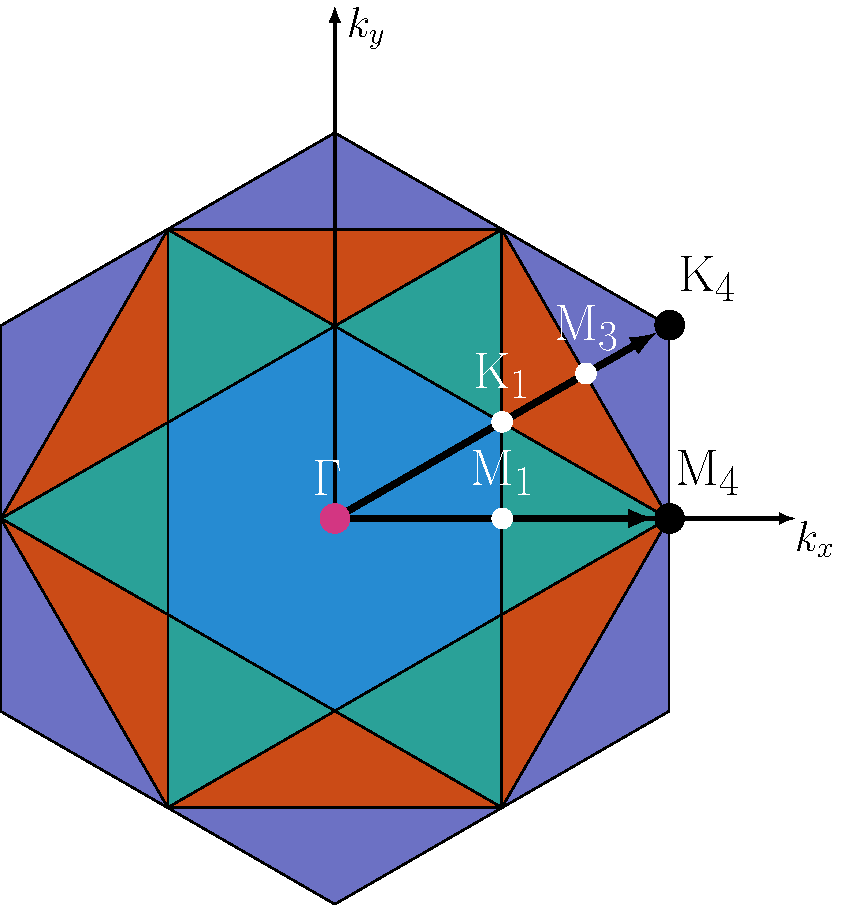
\includegraphics[width=0.6\linewidth]{fig01}
\caption{The two selected in-plane paths along the first four Brillouin zones:
(1) $\Gamma$ to M in the fourth zone (M$_{4}$), and (2) $\Gamma$ to K in the
fourth zone (K$_{4}$).}
\label{fig:brillouin}
\end{figure}

Lastly, we used the DP/EXC code \cite{olevanoDP, reiningEXC} to execute the
calculation of the macroscopic dielectric function ($\epsilon$) and the EEL
spectra for different values of $q$. We obtained converged spectra using 12
shells of reciprocal-space vectors ($\mathbf{G}$), 20 shells of plane waves, and
80 total bands for all methods, except when explicitly noted otherwise.
Local-field effects have been taken into account in every calculation presented
here. The macroscopic dielectric functions and EEL spectra have a 0.6 eV
Gaussian broadening applied to them. Futhermore, in order to simulate the
band-structure stretching, given for instance by GW results \cite{olevano}, a
stretching of 10\,\% was applied to the valence-band energies, and 5\,\% to the
conduction band energies. These parameters and corrections were kept uniform
across all methods studied here. 400 iterations were used for calculations that
make use of the Haydock iterative method.

The DP/EXC code was enabled to use the PETSc \cite{petsc} and SLEPc
\cite{hernandezTOMS05} libraries for diagonalizing \cite{reshetnyakthesis} the
complete excitonic Hamiltonian using MPI parallelism. In fact, it is the
inclusion of these libraries that makes it possible to solve the BSE CP (with
coupling terms included) in a reasonable amount of time. All other calculations
use the OpenMP parallel API, for efficient parallelization and memory use on a
single machine. Appx. \ref{sec:bench} contains detailed computational benchmarks
concerning these calculations.

%%%%%%%%%%%%%%%%%%%%%%%%%%%%%%%%%%%%%%%%%%%%%%%%%%%%%%%%%%%%%%%%%%%%%%%%%%%%%%%%
%%%%%%%%%%%%%%%%%%%%%%%%%%%%%%%%%%%%%%%%%%%%%%%%%%%%%%%%%%%%%%%%%%%%%%%%%%%%%%%%

\section{Results}\label{sec:results}

We calculate the macroscopic dielectric functions and the subsequent EEL spectra
over an energy range between 0 to 45 eV, enough to cover the dispersion behavior
of both the $\pi$ (0--15 eV) and the $\pi + \sigma$ (25--45 eV) plasmons for
each value of momentum transfer $q$. Fig. \ref{fig:brillouin} depicts the two
selected in-plane $q$ paths along which we calculate our results. The $\Gamma
\rightarrow \mathrm{M}_{4}$ path has only variation of $q_{x}$, and passes
through the M point of the first zone. The $\Gamma \rightarrow \mathrm{K}_{4}$
path varies both $q_{x}$ and $q_{y}$ and passes through the K point of the first
zone and the M point of the third zone. As mentioned in Sec. \ref{sec:comp}, we
used 14$\times$14$\times$02 and 12$\times$12$\times$02 \textbf{k}-point grids
for these calculations, allowing us to evaluate the $q$-dependence in steps of
1/14 and/or 1/12 for each path. Shared points between these two grids ($\Gamma$,
M$_{1}$, and M$_{4}$) are virtually identical, meaning that both grids have
acceptable convergence.

The general physical picture of the $q$-dependent plasmon dispersion is as
follows. The shape and intensity of
$\mathrm{Re}\,\epsilon_{\mathrm{M}}(\mathbf{q}, \omega)$ are indicative of the
electron screening behavior, and $\mathrm{Im}\,\epsilon_{\mathrm{M}}(\mathbf{q},
\omega)$ is indicative of interband transitions \cite{marinopoulosPRB04}.
Plasmonic behavior for small values of $q$ are present in the EEL spectrum, with
the thin peaked $\pi$ plasmon appearing around 7 eV, and the much broader $\pi +
\sigma$ plasmon at energies above 25 eV. For values of $q < 1.0$ \r{A}$^{-1}$,
the plasmon criterion is met and the plasmon peak occurs very close to the point
where $\mathrm{Re}\,\epsilon_{\mathrm{M}}(\mathbf{q}, \omega)$ is zero. This
holds true for both the $\Gamma \rightarrow \mathrm{M}$, and $\Gamma
\rightarrow \mathrm{K}$ directions. For larger values of $q$, the plasmon
criterion is no longer met, as $\mathrm{Re}\,\epsilon_{\mathrm{M}}(\mathbf{q},
\omega)$ takes on only positive values; however, the EEL spectrum still presents
defined peaks that correspond to interband transitions only
\cite{marinopoulosPRB04}. This is in accordance to Eq. \ref{eq:eels}, where the
EEL spectra will begin to be less and less affected by the reduced screening of
$\mathrm{Re}\,\epsilon_{\mathrm{M}}(\mathbf{q}, \omega)$, and essentially mimics
$\mathrm{Im}\,\epsilon_{\mathrm{M}}(\mathbf{q}, \omega)$. 

%%%%%%%%%%%%%%%%%%%%%%%%%%%%%%%%%%%%%%%%%%%%%%%%%%%%%%%%%%%%%%%%%%%%%%%%%%%%%%%%

\subsection{The \texorpdfstring{$\pi$}{pi} Plasmon}

\begin{figure}[t]
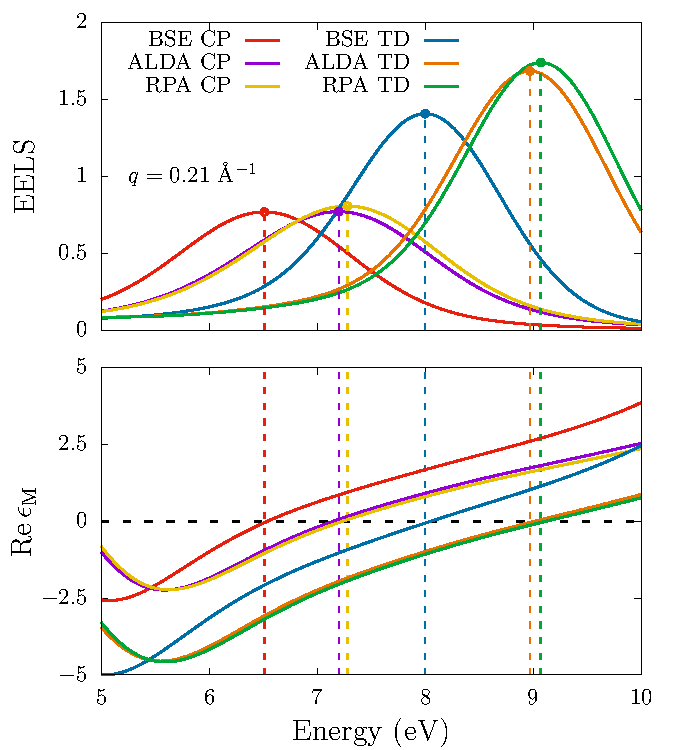
\includegraphics[width=\linewidth]{fig02}
\caption{Top panel: EEL spectra for each method at $q = 0.21$
\r{A}$^{-1}$. Bottom panel: The corresponding real part of the dielectric
function, $\mathrm{Re}\,\epsilon_{\mathrm{M}}$. The plasmon criterion is met for
this low value of $q$; however, the plasmon peak position and intensity varies
widely between each method.}
\label{fig:comparison}
\end{figure}

In Fig. \ref{fig:comparison}, we present a general comparison of the EEL spectra
and macroscopic dielectric function between the different methods, centered
around the energy range of the $\pi$ plasmon. For this low value of $q = 0.21$
\r{A}$^{-1}$, the peak in the EEL spectra meets the aforementioned plasmon
criterion and the plasmon peak energy position matches the zero crossing (from
negative to positive) of $\mathrm{Re}\,\epsilon_{\mathrm{M}}(\mathbf{q},
\omega)$. $\mathrm{Im}\,\epsilon_{\mathrm{M}}(\mathbf{q}, \omega)$ (not shown)
is also very small around this transition point. The plasmon peak is present for
all calculated methods; however, peak position and intensity vary significantly
between them. The predominant difference in peak intensity comes from the
inclusion of the coupling terms in the excitonic Hamiltonian. Methods that
include these (BSE CP, ALDA CP, and RPA CP) have a peak intensity between 0.5
and 1, which compares favorably with experiment \cite{zeppenfeldZP71,
buchnerPSSB77, marinopoulosPRB04}; the remaining methods produce peaks that are
close to twice that value. This relationship also holds true for the energy
range around $\pi + \sigma$ plasmon. The ALDA and RPA calculations yield spectra
that are generally quite similar. We will discuss the peak positions in more
detail below when addressing the $q$-dependent plasmon dispersion.

\begin{figure}[t]
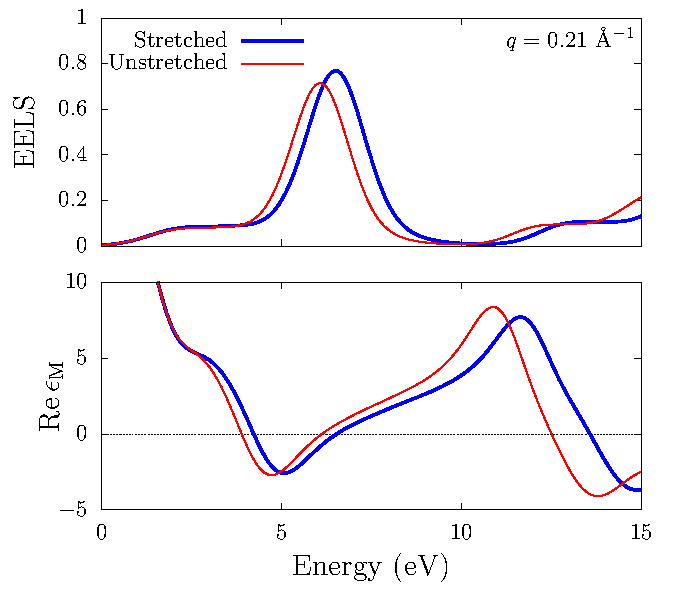
\includegraphics[width=\linewidth]{fig03}
\caption{Top panel: EEL spectra calculated for BSE CP at $q = 0.21$
\r{A}$^{-1}$, with both stretched and unstretched valence and conduction bands.
Bottom panel: The corresponding real part of the dielectric function,
$\mathrm{Re}\,\epsilon_{\mathrm{M}}$. The band stretching causes the spectra
peaks to shift non-rigidly to higher energies.}
\label{fig:stretching}
\end{figure}

Fig. \ref{fig:stretching} depicts the differences introduced into both the EEL
spectrum and the dielectric function when applying valence (conduction) band
stretching of 10\% (5\%). As mentioned above, this band stretching is taking
from GW results \cite{olevano} and compare very well with photoemission
measurements \cite{heskePRB99, marinopoulosPRB04}. Both the EEL spectrum and
dielectric function are shifted towards higher energies; however, the nature of
the stretching causes a redistribution of the band energies, which causes
changes in both the peak position and intensities. Since these values are
applied to the DFT band energies that are used subsequently in the calculation
of the dielectric function, this behavior is consistent across all methods, and
for all calculated values of $q$.

\begin{figure}[b]
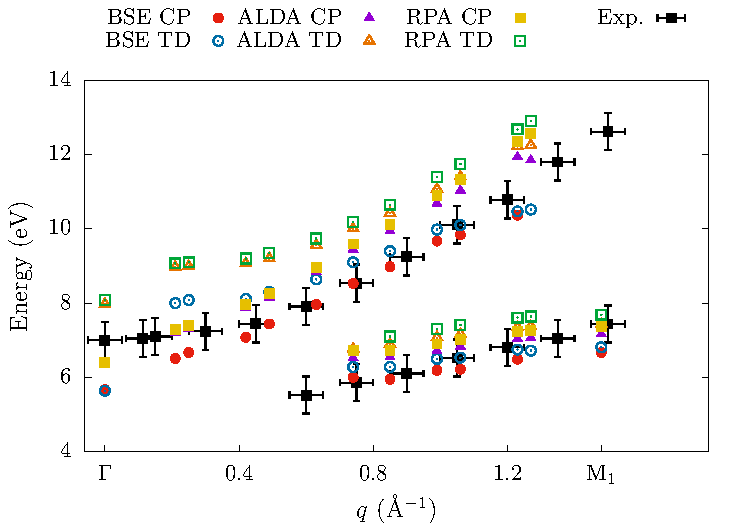
\includegraphics[width=\linewidth]{fig04}
\caption{The $\pi$ plasmon peak position for different values
of $q$ along the $\Gamma \rightarrow \mathrm{M}_{1}$ path for each calculated
method, compared with experimental data \cite{liouPRB15}. The uneven spacing
between the calculated points is due to the use of two \textbf{k}-point grids.}
\label{fig:gm-dispersion}
\end{figure}

In Fig. \ref{fig:gm-dispersion}, we present the $q$-dependent dispersion
behavior of the $\pi$ plasmon, for values of $q$ along the $\Gamma \rightarrow
\mathrm{M}_{1}$ path. Colored points represent the different calculations, while
the black squares are data points from high-resolution EELS measurements
reproduced with permission from Ref. \onlinecite{liouPRB15}. The peaks in the
EEL spectra split into two branches; a main branch that is present for all
values of $q$ with energy values between 7 and 13 eV, and a secondary branch
that begins to appear after $q = 0.6$ \r{A}$^{-1}$ with energy values between 5
and 8 eV. As mentioned above, not all of these points represent plasmon
excitations; in general, points for values of $q > 1.0$ \r{A}$^{-1}$ do not meet
the plasmon criterion and are primarily produced by interband transitions
\cite{marinopoulosPRB04}. However, these points are measured by EELS experiments
and are therefore included in our comparison.

It is evident from the plot that the peak positions vary widely across all
methods, and some general trends can be seen. Calculations that employ the TDA
are generally shifted towards higher energies over their counterparts; thus,
ALDA TD and RPA TD typically present the least similarity with the experimental
data. ALDA CP and RPA CP are quite similar, with ALDA CP presenting some
improvement over RPA CP. Both of these methods tend to have a higher energy
value than the experiment, although they fit well for low values of $q$. The BSE
CP calculation coincides well with the experimental points throughout the entire
$q$-range, but tends to underestimate the energy for large values of $q$. Both
BSE calculations coincide as the value of $q$ increases.

In Fig. \ref{fig:gm-dispersion2}, we focus on the upper branch and compare our
most complete calculation, BSE CP, against three separate experimental EELS
measurements taken from Refs. \onlinecite{zeppenfeldZP71},
\onlinecite{kinyanjuiEPL12}, and \onlinecite{liouPRB15}. These experiments are
mostly consistent amongst each other across the range of $q$-values. Our
calculation yields, in general, quantitatively similar results to the measured
peak values. It is worth noting that, for large $q$-values, our calculation fits
the trend of the ``Zeppenfeld'' data \cite{zeppenfeldZP71} better than the
``Liou'' data \cite{liouPRB15}. Overall, our calculated results can be directly
compared with experiments that span almost five decades, taken by completely
different groups.

\begin{figure}[b]
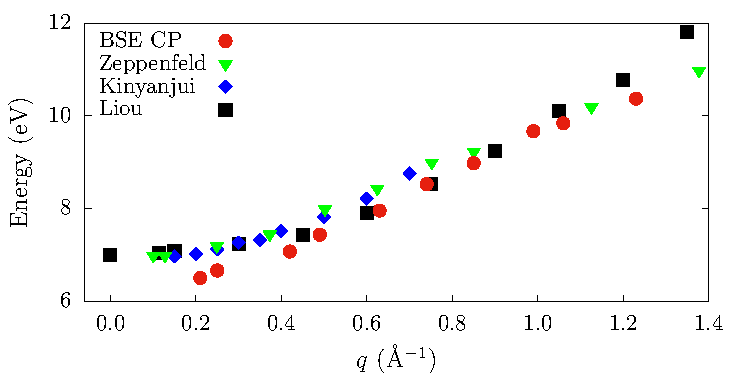
\includegraphics[width=\linewidth]{fig05}
\caption{A more detailed view of the $\pi$ plasmon peak along the $\Gamma
\rightarrow \mathrm{M}_{1}$ path; ``BSE CP'' is our theoretical result (featured
in Fig. \ref{fig:gm-dispersion}), ``Zeppenfeld'' is experimental data from Ref.
\onlinecite{zeppenfeldZP71}, ``Kinyanjui'' from Ref.
\onlinecite{kinyanjuiEPL12}, and ``Liou'' from Ref. \onlinecite{liouPRB15}.
Errorbars have been excluded from the ``Liou'' data for improved legibility.}
\label{fig:gm-dispersion2}
\end{figure}

These trends are in accordance with the approximations implied for each method.
First, taking into account excitons (e-h interactions) causes the peak position
to shift towards lower energies \cite{albrechtPRL98}; second, the inclusion of
the coupling terms in the Hamiltonian further shifts the peak position to lower
energies \cite{olevanoPRL01, gruningNL09}. This explains why BSE CP has the
lowest peak energies, and why RPA TD and ALDA TD have the highest. Furthermore,
the TDA is known to fail at describing plasmonic excitations
\cite{zimmermannPSSB70, caliebePRL00, olevanoPRL01, gruningNL09} due to the
neglected e-h antipairs; thus, for small values of $q$, BSE TD tends to
overestimate the peak energy. However, as the momentum transfer increases the
plasmon dissipates into interband transitions (reducing the number of e-h
antipairs), and the BSE CP and BSE TD calculations begin to coincide. In fact,
this behavior holds true for all methods; in other words, the TDA can accurately
describe the peak positions when plasmon behavior is not expected, or there is
little to no contribution from e-h antipairs.

\begin{figure}[t]
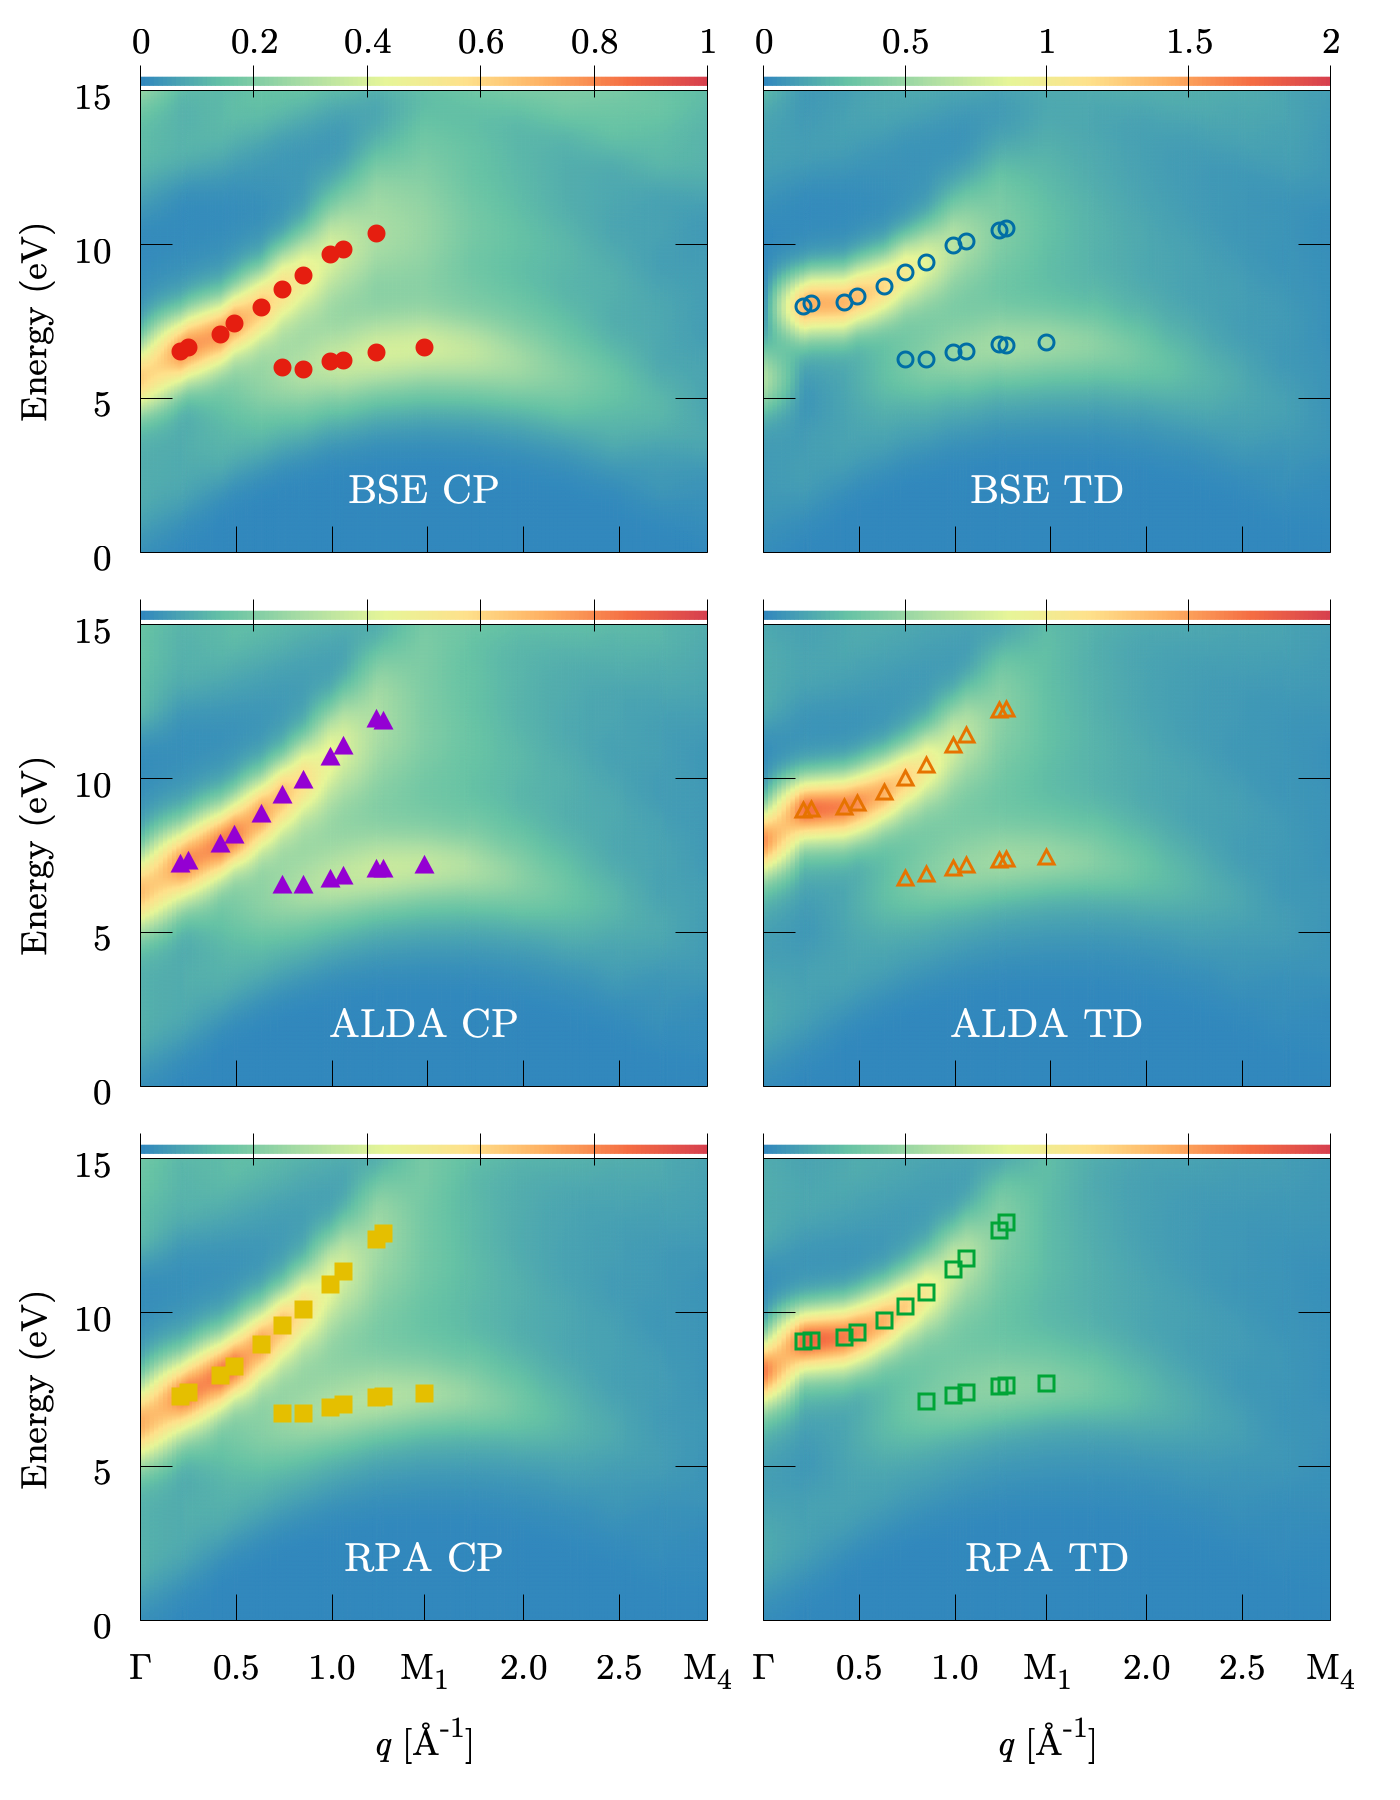
\includegraphics[width=\linewidth]{fig06}
\caption{The EEL spectra for the $\pi$ plasmon region for each method, calculated
for $q$ values along the $\Gamma \rightarrow \mathrm{M}_{4}$ path. The exact
peak positions from Fig. \ref{fig:gm-dispersion} are superimposed on each color
map.}
\label{fig:gm-heatmap_lo}
\end{figure}

In order to elucidate the general trends beyond the experimental data range
(past the M$_{1}$ point in the first Brillouin zone), we extend our calculations
all the way up to the fourth Brillouin zone to the M$_{4}$ point. Fig.
\ref{fig:gm-heatmap_lo} depicts the complete plasmon dispersion for each
calculation, for $q$ values along along the $\Gamma \rightarrow
\mathrm{M}_{4}$ path. The left side of the figure presents the calculated
dispersion including the coupling terms, and the right side with calculations
that neglect them; the EELS intensity scale is located above each column. The
peak positions featured in Fig. \ref{fig:gm-dispersion} are superimposed over
each color map. All methods agree that the upper branch mostly dissipates for
$q$ values beyond M$_{1}$ (1.48 \r{A}$^{-1}$), whilst the lower branch continues
to exist throughout the range. As mentioned above, the behavior of both
$\epsilon_{1}$ and $\epsilon_{2}$, which does not conform to the plasmon
criterion for these high $q$ values, indicate that these peaks are primarily due
to interband transitions and are not plasmons. Our predictions also show that
the lower branch presents negative dispersion after M$_{1}$, appears to return
to lower energies rather than continuing upwards. Confirmation of this trend
will require future experimental measurements taken at similarly high values of
$q$. While these plots are very useful to discern trends, they show that the
differences between each method are subtle, and must be analyzed in closer
detail as we have in Figs. \ref{fig:gm-dispersion} and \ref{fig:gm-dispersion2}.

\begin{figure}[b]
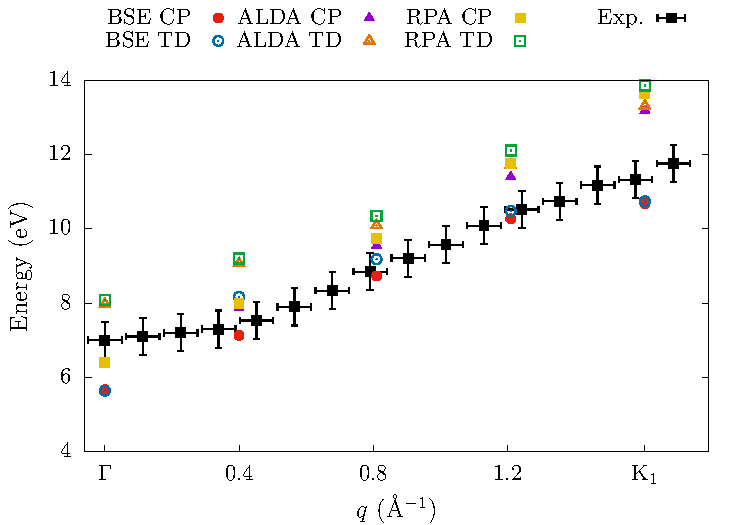
\includegraphics[width=\linewidth]{fig07}
\caption{The $\pi$ plasmon peak position for different values of $q$ along the
$\Gamma \rightarrow \mathrm{K}_{1}$ path for each calculated method, compared
with experimental data from Ref. \onlinecite{liouPRB15}.}
\label{fig:gk-dispersion}
\end{figure}

Likewise, we conduct a similar analysis for the $\Gamma \rightarrow
\mathrm{K}_{1}$ path in Fig. \ref{fig:gk-dispersion}. For these values of
$q$, the spectra is dominated by a single peak with energy positions ranging
from 7 to 12 eV, where the classical plasmonic behavior is lost after $q\approx
1.00$ \r{A}$^{-1}$. Once again, our calculations confirm the strong dispersion
of the peak position. ALDA TD and RPA TD significantly overestimate the peak
energy position, and CP and TD calculations begin to coincide for increasing
momentum transfer. BSE CP yields good agreement with experiment throughout the
range. We also extend our calculations for increasing $q$ values into the fourth
Brillouin zone K$_{4}$ point. Fig. \ref{fig:gk-heatmap_lo} features the entire
range for all calculated methods. In general, all methods feature a well
resolved peak at low values, that broadens and decreases in intensity for
increasing values of $q$. The dispersion is much more linear when compared to
the $\Gamma \rightarrow \mathrm{M}_{4}$ path; however, both BSE methods have a
slight decrease in energy at large values of $q$.

\begin{figure}[t]
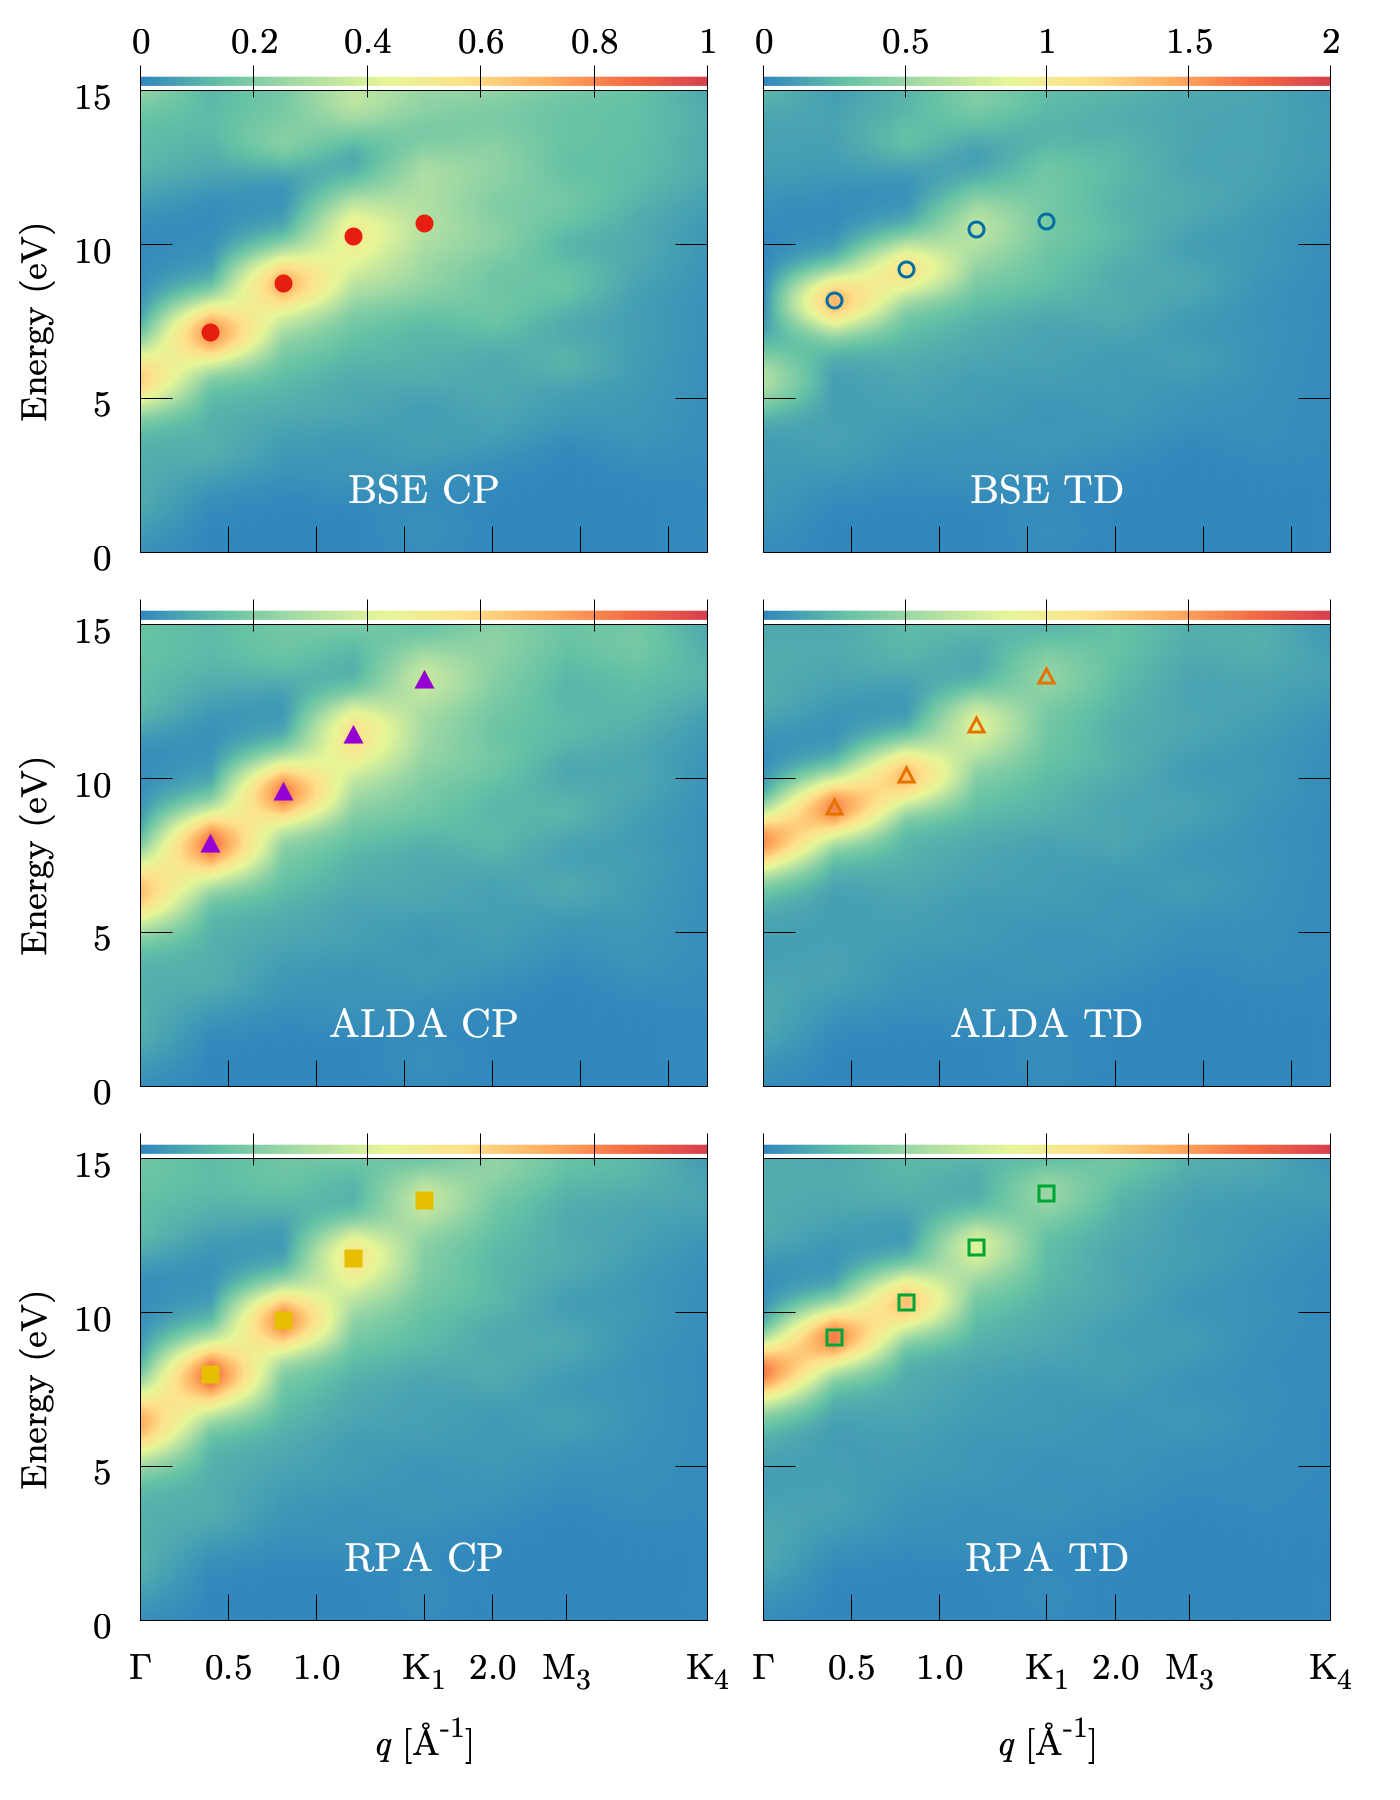
\includegraphics[width=\linewidth]{fig08}
\caption{The EEL spectra for the $\pi$ plasmon region for each method,
calculated for $q$ values along the $\Gamma \rightarrow \mathrm{K}_{4}$ path.
The exact peak positions from Fig. \ref{fig:gk-dispersion} are superimposed on
each color map.}
\label{fig:gk-heatmap_lo}
\end{figure}

%%%%%%%%%%%%%%%%%%%%%%%%%%%%%%%%%%%%%%%%%%%%%%%%%%%%%%%%%%%%%%%%%%%%%%%%%%%%%%%%

\subsection{The \texorpdfstring{$\pi + \sigma$}{pi + sigma} Plasmon}

Our theoretical calculations do not have to be limited to only the low energy
range used in the experiments. The $\pi + \sigma$ plasmon that occurs in the 20
to 40 eV range retains its plasmonic character for momentum values up to $q
\approx 1.5$ \r{A}$^{-1}$. Figs. \ref{fig:gm-heatmap_hi} and
\ref{fig:gk-heatmap_hi} depict the $q$-dependent dispersion in the 15 to 45 eV
energy range for each calculated method, along the $\Gamma \rightarrow
\mathrm{M}_{4}$ and $\Gamma \rightarrow \mathrm{K}_{4}$ paths, respectively. One
crucial remark about these results concerns the number of bands included in each
calculation; with the exception of the BSE CP calculation, all methods include
80 total bands in order to obtain well-converged results over the full energy
range. The BSE CP calculation, due to the considerable computational expense of
diagonalizing the complete Hamiltonian, only includes 20 total bands which is
enough to obtain convergence for the low energy range of the $\pi$ plasmon, but
not enough for the high energy range presented here. Therefore, this data cannot
be used for quantitative analysis, although the general trend can be readily
visualized.

\begin{figure}[b]
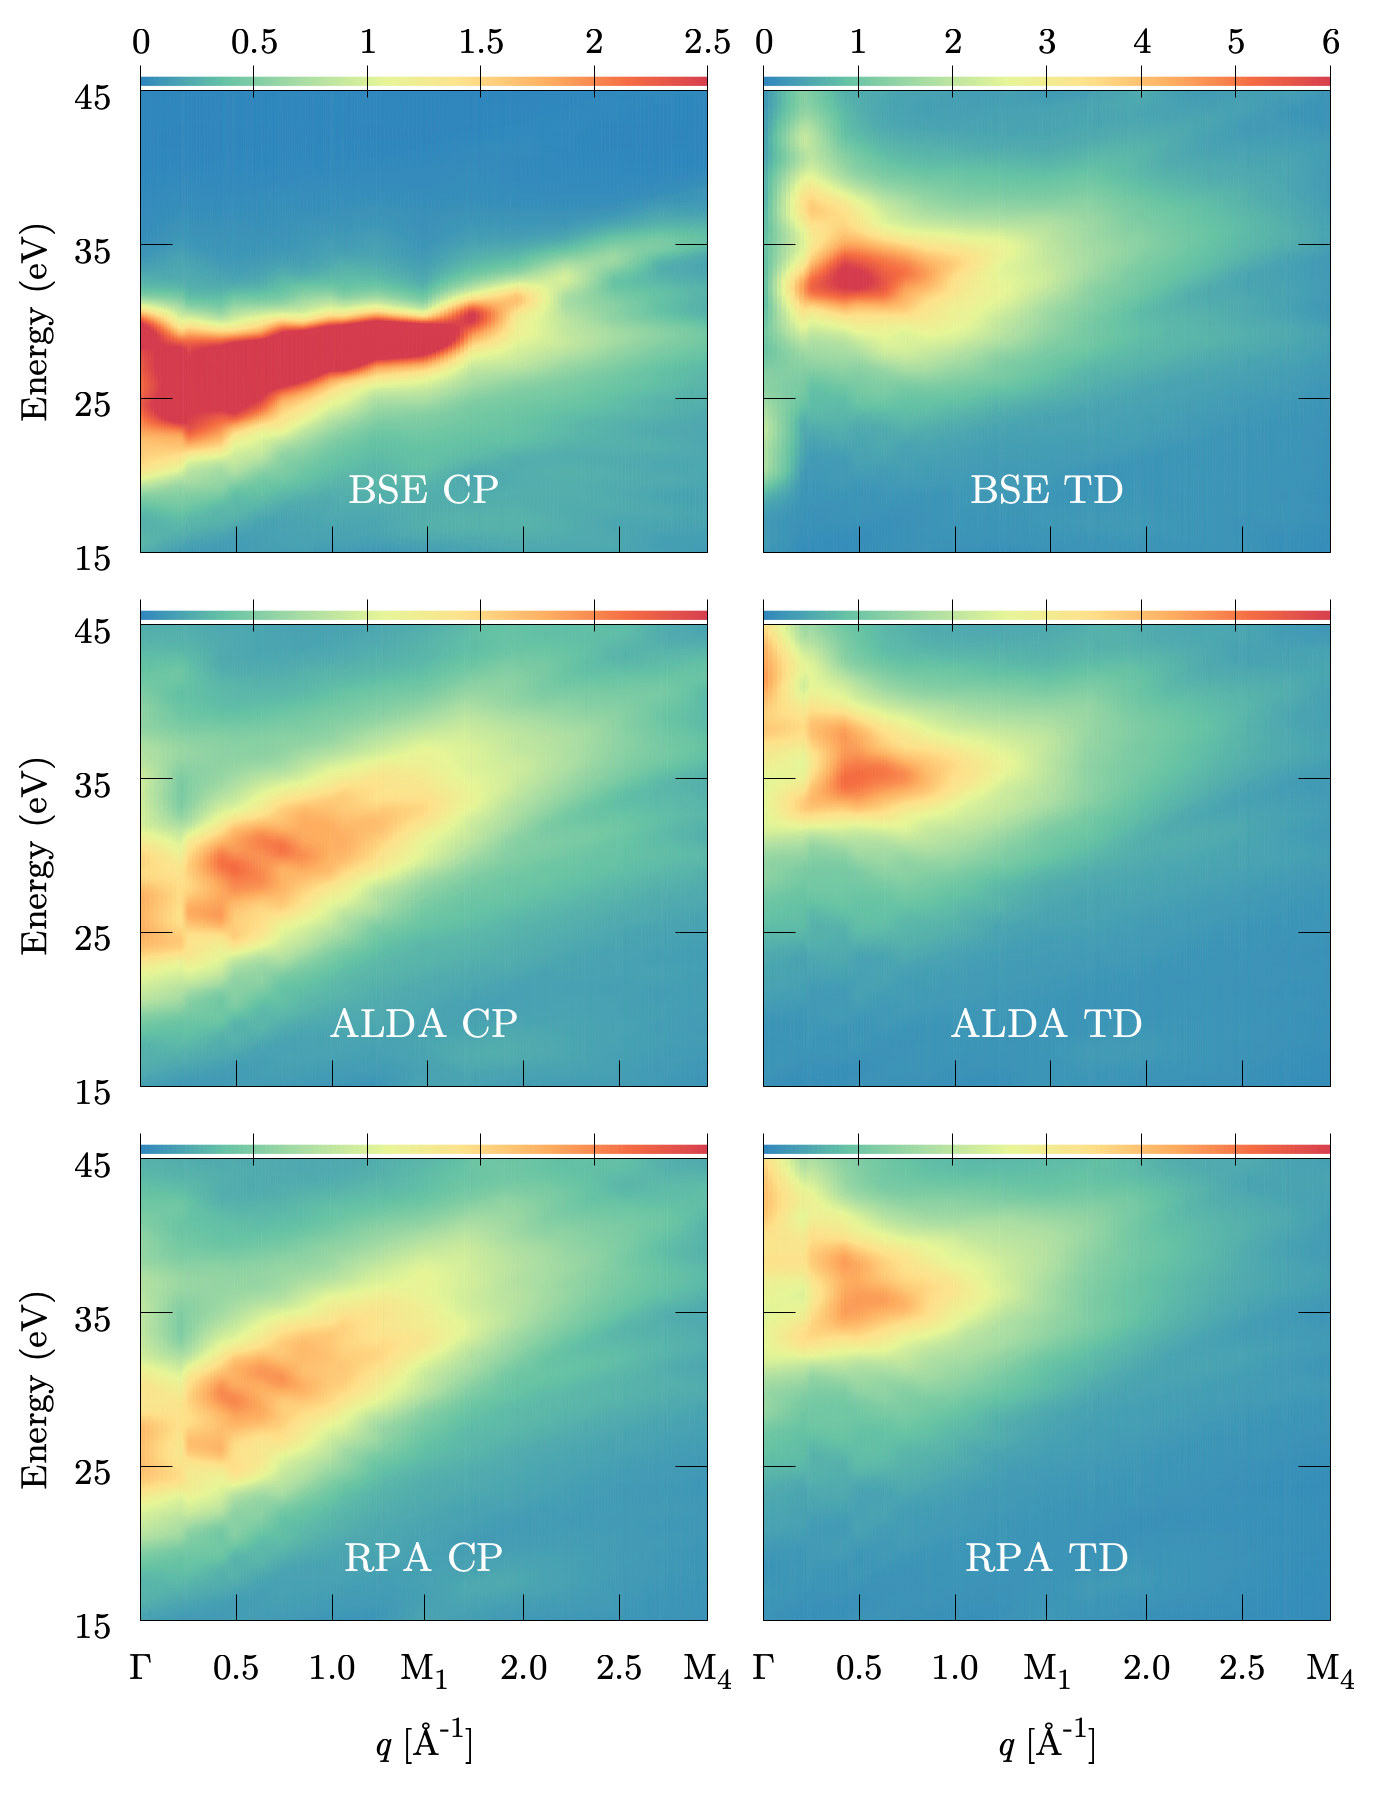
\includegraphics[width=\linewidth]{fig09}
\caption{The EEL spectra for the $\pi + \sigma$ plasmon region for each method,
calculated for $q$ values along the $\Gamma \rightarrow \mathrm{M}_{4}$ path.}
\label{fig:gm-heatmap_hi}
\end{figure}

Available experimental data \cite{zeppenfeldZP71, buchnerPSSB77,
marinopoulosPRB04} shows that the $\pi + \sigma$ plasmon peak, for $q = 0$
\r{A}$^{-1}$, is between 25 to 30 eV. As the value of $q$ increases, the peak
widens, decreases slightly in intensity, and moves towards higher energies. We
find that this behavior is well reproduced with methods that include the
coupling terms in the excitonic Hamiltonian, and our calculations predict that
this plasmon continues to increase in width and decrease in intensity until
almost fully dissipating at large values of $q$. The BSE CP calculation, as
mentioned above, does not have enough bands included in order to reproduce the
fine features and intensity of the peak. However, the general trend is the same.
On the other hand, methods that use the Tamm-Dancoff approximation and neglect
these coupling terms tell a different story altogether. These methods tend to
substantially overestimate the peak energy position for low values of $q$, have
around twice the peak intensity, and very rapidly diminish in intensity towards
medium values of $q$. This behavior does not fit the aforementioned experimental
data at all. The dispersive behavior of the $\pi + \sigma$ plasmon is very
similar for both the $\Gamma \rightarrow \mathrm{M}_{4}$ and $\Gamma \rightarrow
\mathrm{K}_{4}$ paths.

\begin{figure}[t]
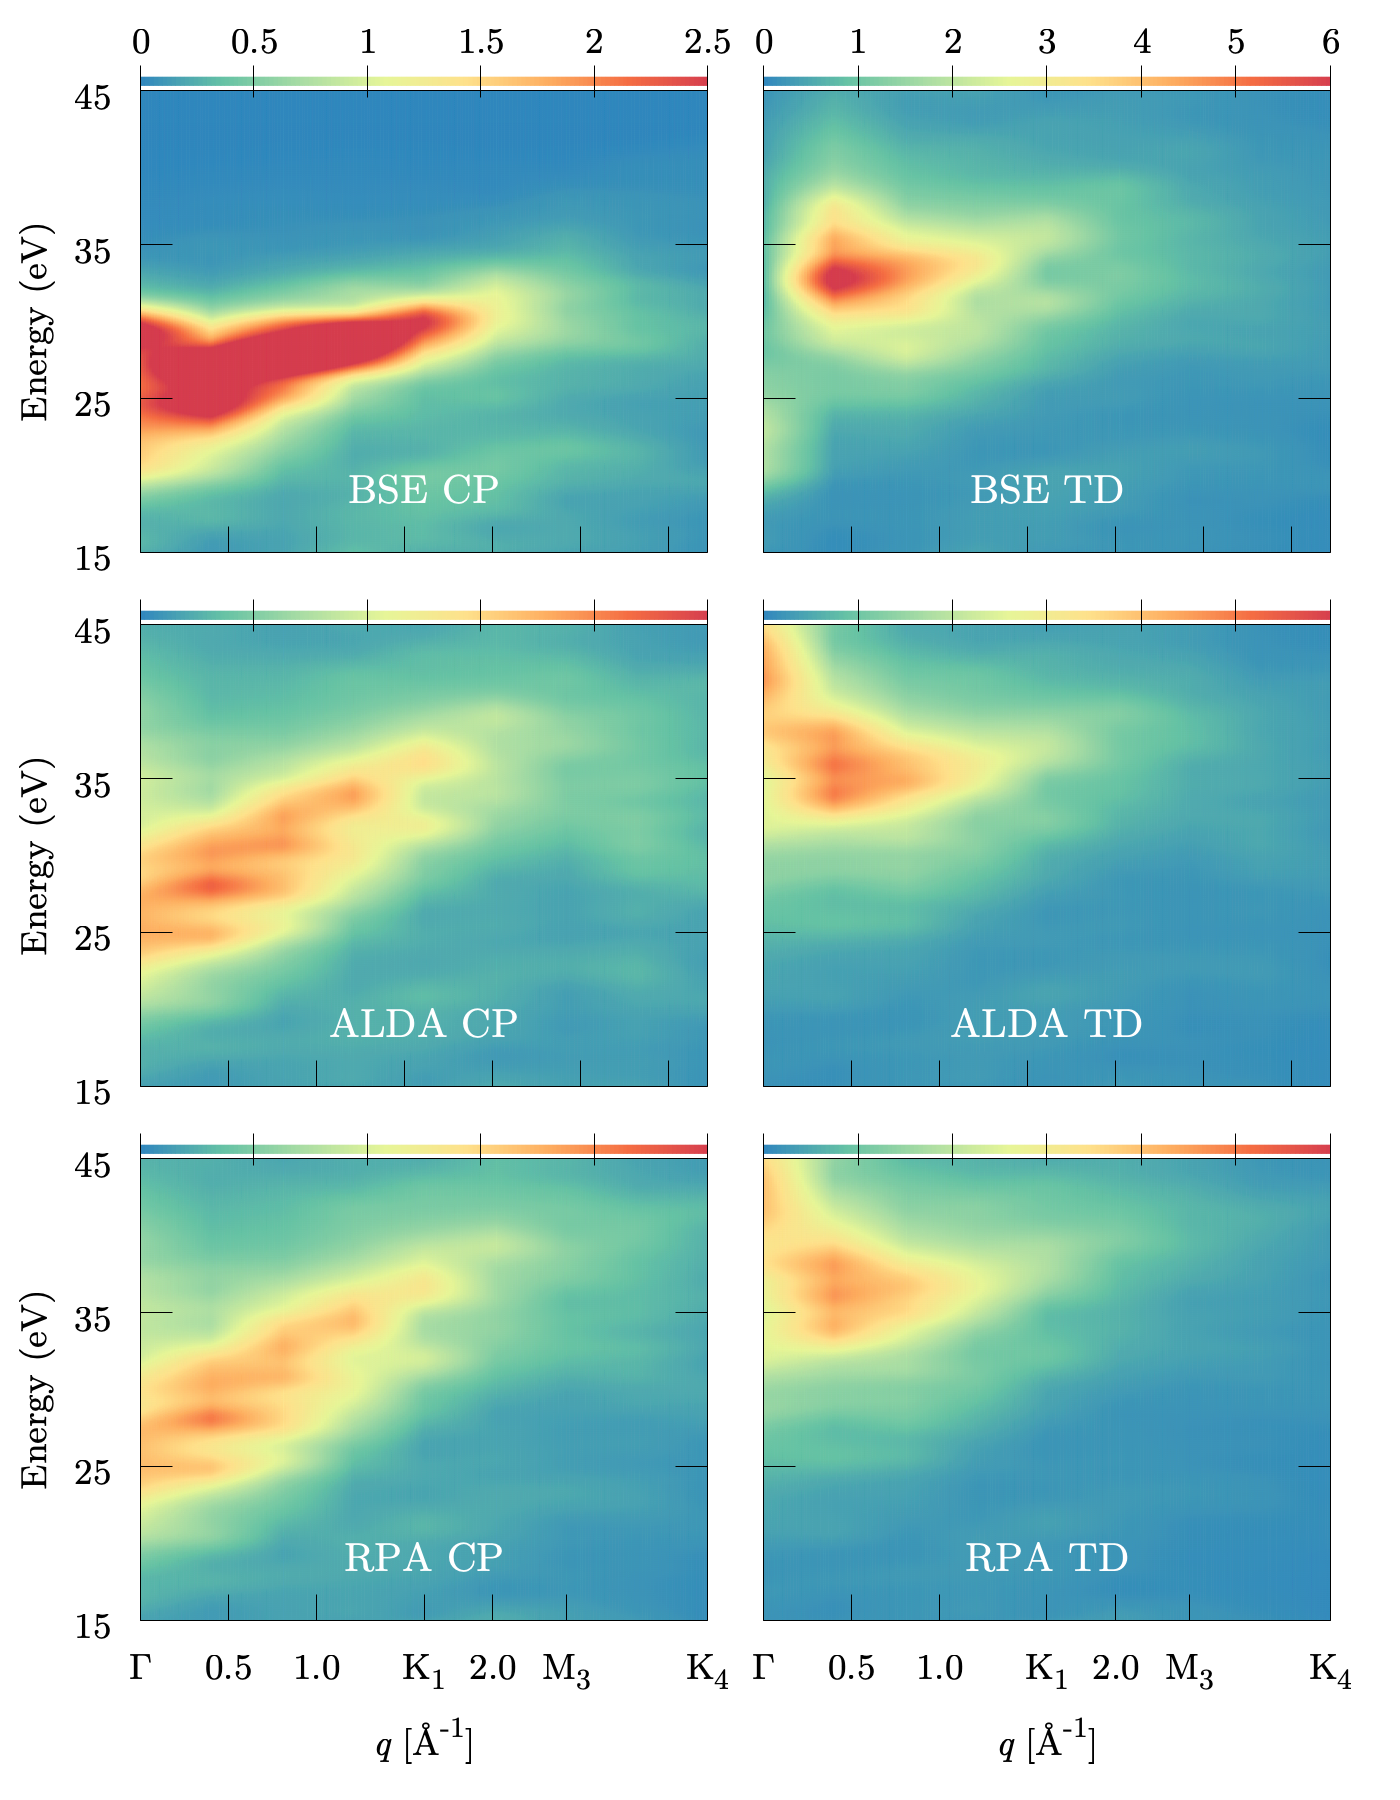
\includegraphics[width=\linewidth]{fig10}
\caption{The EEL spectra for the $\pi + \sigma$ plasmon region for each method,
calculated for $q$ values along the $\Gamma \rightarrow \mathrm{K}_{4}$ path.}
\label{fig:gk-heatmap_hi}
\end{figure}

These plots mark a striking visual difference between using the full excitonic
Hamiltonian and the TDA; the latter is simply not well-suited for describing
plasmon excitations. Overall, the BSE offers the best agreement with experiment,
and can accurately describe both exciton and plasmon excitations when used with
the full Hamiltonian; the coupling terms are crucial for accurately describing
plasmon behavior.

%%%%%%%%%%%%%%%%%%%%%%%%%%%%%%%%%%%%%%%%%%%%%%%%%%%%%%%%%%%%%%%%%%%%%%%%%%%%%%%%
%%%%%%%%%%%%%%%%%%%%%%%%%%%%%%%%%%%%%%%%%%%%%%%%%%%%%%%%%%%%%%%%%%%%%%%%%%%%%%%%

\section{Conclusions}\label{sec:conclusions}

We carried out a systematic study of the macroscopic dielectric function and EEL
spectra for graphite for an energy range encompassing the $\pi$ and $\pi +
\sigma$ plasmons, comparing \emph{ab initio} TDDFT and BSE methods. We selected
graphite as a good benchmark case due to the extensive theoretical and
experimental work available. Our results coincide with previous literature
(where available), and offer quantitative agreement with experiment. Using two
non-equivalent momentum paths spanning the first four Brillouin zones, we are
able to deduce the importance of the coupling terms in the excitonic Hamiltonian
for describing plasmon excitations. The TDA, while numerically efficient, cannot
reproduce many key features in the experimental EEL spectra, nor the plasmon
dispersion behavior. Access to high-resolution EELS measurements around the
$\pi$ plasmon allow us to compare subtle details, while predictive calculations
of the $\pi + \sigma$ plasmon reveal important trends for each method.

Overall, we provide an overview of \emph{ab initio} methods that are considered
state-of-the-art at describing the optoelectronic properties of solid state
systems. We have applied these methods on graphite, which offers an excellent
benchmark material for this type of study. We are confident this work can be
used as reference for future work. The knowledge of the inverse dielctric
function for the wide range of momentum transfer and energy (beyond the
experimental range available today) that we provide, gives useful insights also
for other methods which are intrinsically based on the concept of Coulomb
screening, like many-body GW (and beyond GW) approaches \cite{rodlPRB17,
luciabook}, hybrid functionals in DFT \cite{krukauJCP06}, or Dynamical Mean
Field Theory \cite{biermannJPCM14}.

Finally, as the benchmarks (see Appx. \ref{sec:bench}) clearly show, the
significant computational cost of BSE CP may not be necessarily warranted for
every situation. The very low computational expense of the TDDFT methods
compared to the BSE, make them an attractive alternative when the coupling terms
are the determining factors for a calculation. In summary, these methods should
always be applied judiciously and their use evaluated on a case by case basis.

%%%%%%%%%%%%%%%%%%%%%%%%%%%%%%%%%%%%%%%%%%%%%%%%%%%%%%%%%%%%%%%%%%%%%%%%%%%%%%%%
%%%%%%%%%%%%%%%%%%%%%%%%%%%%%%%%%%%%%%%%%%%%%%%%%%%%%%%%%%%%%%%%%%%%%%%%%%%%%%%%

\section{Acknowledgments}

The authors would like to thank S. C. Liou for graciously contributing the
experimental data featured in this work, and also M. Gatti and I. Reshetnyak for
fruitful discussion. The authors thankfully acknowledge the computer resources,
technical expertise, and support provided by the Laboratorio Nacional de
Superc\'omputo del Sureste de M\'exico, a member of the CONACYT network of
national laboratories. S. M. Anderson acknowledges partial support for this
project from CONACYT-M\'exico scholarship 349278.

%%%%%%%%%%%%%%%%%%%%%%%%%%%%%%%%%%%%%%%%%%%%%%%%%%%%%%%%%%%%%%%%%%%%%%%%%%%%%%%%
%%%%%%%%%%%%%%%%%%%%%%%%%%%%%%%%%%%%%%%%%%%%%%%%%%%%%%%%%%%%%%%%%%%%%%%%%%%%%%%%

\appendix
\section{Benchmarks}\label{sec:bench}

During the course of this study, we were able to gather a significant amount of
real-world performance data for the purpose of benchmarking the different
calculations. Table \ref{tab:times} presents the most general time metrics for
each of the different methods featured in this work; these values include the
entire calculation time, from reading the input files to writing the final
datasets. The standard deviation ($\sigma$) for each value was determined from
the multiple calculations required for each grid of \textbf{k}-points. In
general, $\sigma$ merely represents the normal fluctuations in clock speed and
available resources that occur in any computing system. The compute nodes used
in these benchamarks consist of three Intel Xeon E7-8860v3 platforms with clock
speeds of 2.20 GHz. Each node has four processors for a total of 64 cores and 3
TB of DDR4 RAM memory.

\begin{table}[t]
\caption{Duration in minutes for each of the different levels of approximation
for the 14$\times$14$\times$02 (392) grid of \textbf{k}-points, alongside the
standard deviation and the number of cores used. A total of 20 bands were
included in the calculation.}
\label{tab:times}
\begin{ruledtabular}
\begin{tabular}{ r c c c c c }
Method & Duration\,(min) & $\sigma$\,(min) & Cores\\
\hline
BSE CP  & 20559.13       & 472.52          & 64\\
BSE TD  &    40.05       &   0.32          & 64\\
ALDA CP &     7.67       &   1.10          & 32\\
ALDA TD &     1.90       &   0.17          & 32\\
RPA CP  &     3.35       &   0.43          & 32\\
RPA TD  &     1.63       &   0.25          & 32
\end{tabular}
\end{ruledtabular}
\end{table}

These benchmarks make it clear that solving the BSE the full excitonic
Hamiltonian implies an enormous leap in computational time; for this particular
grid, the time is up to 5 orders of magnitude larger. Fortunately, this time can
be greatly reduced by further parallelizing the number of \textbf{k}-points over
more cores. As mentioned above, each of our compute nodes has 64 cores allowing
us to parallelize over 192 cores total. Table \ref{tab:cores} presents the
duration (in days) of the full excitonic calculation for the
14$\times$14$\times$02 grid as a function of the number of cores. The total time
is reduced by around 50\% by doubling the number of cores from 64 to 128 (at
which point we more or less reach the scalability range of our code). This study
is obviously not exhaustive as the number of cores used was not optimal; the
14$\times$14$\times$02 has 392 \textbf{k}-points which is not evenly divisible
by 64, 128, or 192. However, we can clearly see that the parallelization is
still very effective across two nodes, probably reaching peak efficiency at 98
cores with 4 \textbf{k}-points per core. However, as these numbers were obtained
over the course of many trials and for such long calculations, emphasis was
given on the number of simultaneous calculations possible rather than the most
optimized parallelization for each one.

\begin{table}[t]
\caption{Duration in days for each of the different levels of approximation
for the 14$\times$14$\times$02 (392) grid of \textbf{k}-points, alongside the
standard deviation and the number of cores used. A total of 20 bands were
included in the calculation.}
\label{tab:cores}
\begin{ruledtabular}
\begin{tabular}{ r c c c c }
Cores & Duration\,(Days) & $\sigma$\,(Days) & \textbf{k}-points\\
\hline
 64   & 14.3             & 0.33             & 392 \\
128   &  7.4             & 0.00             & 392 \\
192   &  7.8             & 0.21             & 392
\end{tabular}
\end{ruledtabular}
\end{table}

Lastly, the full excitonic calculation also has significant memory requirements
that must be taken into consideration. The memory required for storing the
excitonic Hamiltonian (in GB) can be calculated using the following expression,
\begin{equation}\label{eq:mem}
(k_{x}\times k_{y}\times k_{z}\times N_{v}\times N_{c})^{2} \times
\frac{8\, \mathrm{bytes}}{1024^{3}},
\end{equation}
where $k_{x}$, $k_{y}$, and $k_{z}$ define the \textbf{k}-point grid, and
$N_{v}$ and $N_{c}$ are the number of valence and conduction bands,
respectively. Fig. \ref{fig:bands} depicts the relation from Eq. \eqref{eq:mem}
(solid red line) using the left-side axis. The size of the excitonic Hamiltonian
was around 300 GB for this work, with 80 total bands included for most
calculations. The blue dots and dotted line are the raw calculation times (in
hours) and the quartic fit for the BSE TD method. The reduced Hamiltonian in the
TDA, coupled with the very efficient Haydock iterative scheme vastly reduces the
calculation time compared to the BSE with the full Hamiltonian. However,
calcultion time still increases very rapidly with the number of bands; which is
particularly troublesome for systems with spectral features present at high
energies. Unfortunately, we are not able to provide this same benchmark for the
BSE CP method, as calculation time became unwieldy above 20 total bands.

\begin{figure}[t]
{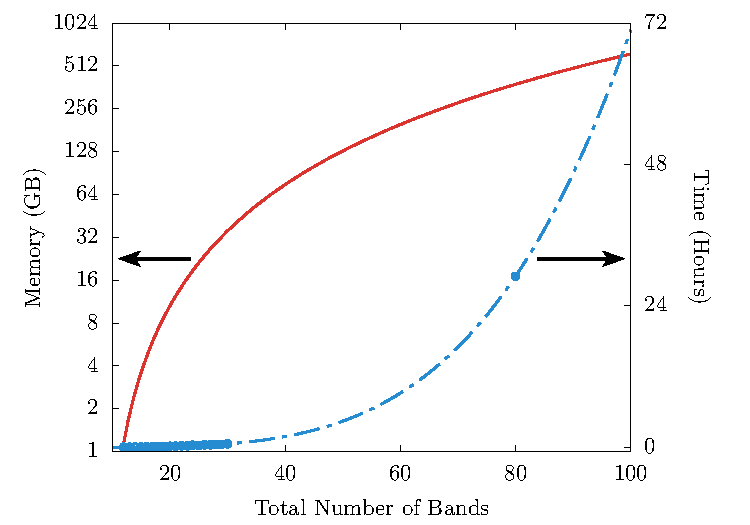
\includegraphics[width=\linewidth]{fig11}}
\caption{Memory usage (in GB) as a function of the total number of
bands (red solid line, left-hand scale), and calculation time as a function of
the total number bands included in the BSE TD method for the 14x14x02
\textbf{k}-point grid, parallelized over 64 cores (blue circles, right-hand
scale). The blue dotted line is a quartic fit, where $f(N) =
7.082\times10^{-7}N^{4}$ in hours.}
\label{fig:bands}
\end{figure}

%%%%%%%%%%%%%%%%%%%%%%%%%%%%%%%%%%%%%%%%%%%%%%%%%%%%%%%%%%%%%%%%%%%%%%%%%%%%%%%%
%%%%%%%%%%%%%%%%%%%%%%%%%%%%%%%%%%%%%%%%%%%%%%%%%%%%%%%%%%%%%%%%%%%%%%%%%%%%%%%%

\bibliographystyle{unsrt}
% \bibliography{refs}

\begin{thebibliography}{10}

\bibitem{hohenbergPR64}
P.~Hohenberg and W.~Kohn.
\newblock Inhomogeneous electron gas.
\newblock {\em Phys. Rev.}, 136(3B):B864, 1964.

\bibitem{kohnPR65}
W.~Kohn and L.~J. Sham.
\newblock Self-consistent equations including exchange and correlation effects.
\newblock {\em Phys. Rev.}, 140(4A):A1133--A1138, November 1965.

\bibitem{rungePRL84}
E.~Runge and E.~K.~U. Gross.
\newblock Density-{Functional} {Theory} for {Time}-{Dependent} {Systems}.
\newblock {\em Phys. Rev. Lett.}, 52(12):997--1000, March 1984.

\bibitem{onidaRMP02}
G.~Onida, L.~Reining, and A.~Rubio.
\newblock Electronic excitations: density-functional versus many-body
  green's-function approaches.
\newblock {\em Rev. Mod. Phys.}, 74(2):601, 2002.

\bibitem{gavrilenkoPRB97}
V.~I. Gavrilenko and F.~Bechstedt.
\newblock Optical functions of semiconductors beyond density-functional theory
  and random-phase approximation.
\newblock {\em Phys. Rev. B}, 55(7):4343--4352, February 1997.

\bibitem{fetterbook72}
A.~L. Fetter and J.~D. Walecka.
\newblock {\em Quantum {Theory} of {Many} {Particle} {Systems}}, volume~25.
\newblock McGraw-Hill, Inc., 1972.

\bibitem{hedinPR65}
L.~Hedin.
\newblock New method for calculating the one-particle {Green}'s function with
  application to the electron-gas problem.
\newblock {\em Phys. Rev.}, 139(3A):A796--A823, 1965.

\bibitem{salpeterPR51}
E.~E. Salpeter and H.~A. Bethe.
\newblock A relativistic equation for bound-state problems.
\newblock {\em Phys. Rev.}, 84(6):1232, 1951.

\bibitem{abrikosovbook65}
A.~A. Abrikosov, L.~P. Gorlcov, and I.~E. Illyaloslinski.
\newblock {\em Methods of {Quantum} {Field} {Theory} in {Statistical}
  {Physics}}, volume~4 of {\em Quantum {Field} {Theoretical} {Methods} in
  {Statistical} {Physics}}.
\newblock Pergamon Press, 1965.

\bibitem{shamPR66}
L.~J. Sham and T.~M. Rice.
\newblock Many-{Particle} {Derivation} of the {Effective}-{Mass} {Equation} for
  the {Wannier} {Exciton}.
\newblock {\em Phys. Rev.}, 144(2):708--714, April 1966.

\bibitem{hankePRB80}
W.~Hanke and L.~J. Sham.
\newblock Many-particle effects in the optical spectrum of a semiconductor.
\newblock {\em Phys. Rev. B}, 21(10):4656, 1980.

\bibitem{shirleyPRL93}
E.~L. Shirley and S.~G. Louie.
\newblock Electron excitations in solid {C} 60 : {Energy} gap, band
  dispersions, and effects of orientational disorder.
\newblock {\em Phys. Rev. Lett.}, 71(1):133--136, July 1993.

\bibitem{albrechtPRB97}
S.~Albrecht, G.~Onida, and L.~Reining.
\newblock Ab initio calculation of the quasiparticle spectrum and excitonic
  effects in {Li$_{2}$O}.
\newblock {\em Phys. Rev. B}, 55(16):10278--10281, April 1997.

\bibitem{benedictPRL98}
L.~X. Benedict, E.~L. Shirley, and R.~B. Bohn.
\newblock Optical {Absorption} of {Insulators} and the {Electron}-{Hole}
  {Interaction}: {An} {Ab} {Initio} {Calculation}.
\newblock {\em Phys. Rev. Lett.}, 80(20):4514--4517, May 1998.

\bibitem{benedictPRB99}
L.~X. Benedict and E.~L. Shirley.
\newblock Ab initio calculation of {$\epsilon_{2}\omega$} including the
  electron-hole interaction: {Application} to {GaN} and {CaF$_{2}$}.
\newblock {\em Phys. Rev. B}, 59(8):5441, 1999.

\bibitem{benedictPRB03}
L.~X. Benedict, A.~Puzder, A.~J. Williamson, J.~C. Grossman, G.~Galli, J.~E.
  Klepeis, J.-Y. Raty, and O.~Pankratov.
\newblock Calculation of optical absorption spectra of hydrogenated {Si}
  clusters: {Bethe}-{Salpeter} equation versus time-dependent local-density
  approximation.
\newblock {\em Phys. Rev. B}, 68(8):085310, August 2003.

\bibitem{palummoJPCM04}
M.~Palummo, O.~Pulci, R.~Del~Sole, A.~Marini, P.~Hahn, W.~G. Schmidt, and
  F.~Bechstedt.
\newblock The {Bethe}-{Salpeter} equation: a first-principles approach for
  calculating surface optical spectra.
\newblock {\em J. Phys. Condens. Matter}, 16(39):S4313--S4322, October 2004.

\bibitem{sittPRA07}
A.~Sitt, L.~Kronik, S.~Ismail-Beigi, and J.~R. Chelikowsky.
\newblock Excited-state forces within time-dependent density-functional theory:
  {A} frequency-domain approach.
\newblock {\em Phys. Rev. A}, 76(5):054501, November 2007.

\bibitem{ramosPRB08}
L.~E. Ramos, J.~Paier, G.~Kresse, and F.~Bechstedt.
\newblock Optical spectra of {Si} nanocrystallites: {Bethe}-{Salpeter} approach
  versus time-dependent density-functional theory.
\newblock {\em Phys. Rev. B}, 78(19):195423, November 2008.

\bibitem{roccaJCP10}
D.~Rocca, D.~Lu, and G.~Galli.
\newblock Ab initio calculations of optical absorption spectra: {Solution} of
  the {Bethe}-{Salpeter} equation within density matrix perturbation theory.
\newblock {\em J. Chem. Phys.}, 133(16):164109, 2010.

\bibitem{garciaJCP11}
J.~M. Garcia-Lastra, J.~D. Bass, and K.~S. Thygesen.
\newblock Communication: {Strong} excitonic and vibronic effects determine the
  optical properties of {Li}$_{2}$ {O}$_{2}$.
\newblock {\em J. Chem. Phys.}, 135(12):121101, September 2011.

\bibitem{gruningCMS11}
M.~Gr{\"u}ning, A.~Marini, and X.~Gonze.
\newblock Implementation and testing of {Lanczos}-based algorithms for
  random-phase approximation eigenproblems.
\newblock {\em Comput. Mater. Sci}, 50(7):2148--2156, May 2011.

\bibitem{gattiPRB13}
M.~Gatti and F.~Sottile.
\newblock Exciton dispersion from first principles.
\newblock {\em Phys. Rev. B}, 88(15):155113, October 2013.

\bibitem{onidaPRL95}
G.~Onida, L.~Reining, R.~W. Godby, R.~Del~Sole, and W.~Andreoni.
\newblock Ab {Initio} {Calculations} of the {Quasiparticle} and {Absorption}
  {Spectra} of {Clusters}: {The} {Sodium} {Tetramer}.
\newblock {\em Phys. Rev. Lett.}, 75(5):818--821, July 1995.

\bibitem{albrechtPRL98}
S.~Albrecht, L.~Reining, R.~Del~Sole, and G.~Onida.
\newblock Ab initio calculation of excitonic effects in the optical spectra of
  semiconductors.
\newblock {\em Phys. Rev. Lett.}, 80(20):4510--4513, May 1998.

\bibitem{benedictPRB98}
Lorin~X. Benedict, Eric~L. Shirley, and Robert~B. Bohn.
\newblock Theory of optical absorption in diamond, {Si}, {Ge}, and {GaAs}.
\newblock {\em Phys. Rev. B}, 57(16):R9385--R9387, April 1998.

\bibitem{rohlfingPRL98b}
M.~Rohlfing and S.~G. Louie.
\newblock Electron-hole excitations in semiconductors and insulators.
\newblock {\em Phys. Rev. Lett.}, 81(11):2312--2315, September 1998.

\bibitem{haydockJPC72}
R.~Haydock, V.~Heine, and M.~J. Kelly.
\newblock Electronic structure based on the local atomic environment for
  tight-binding bands.
\newblock {\em J. Phys. C: Solid State Phys.}, 5(20):2845--2858, October 1972.

\bibitem{haydockCPC80}
R.~Haydock.
\newblock The recursive solution of the {Schr{\"o}dinger} equation.
\newblock {\em Comput. Phys. Commun.}, 20(1):11--16, September 1980.

\bibitem{roccaJCP08}
D.~Rocca, R.~Gebauer, Y.~Saad, and S.~Baroni.
\newblock Turbo charging time-dependent density-functional theory with
  {Lanczos} chains.
\newblock {\em J. Chem. Phys.}, 128(15):154105, April 2008.

\bibitem{lopezPRL06}
M.~Lopez~del Puerto, M.~L. Tiago, and J.~R. Chelikowsky.
\newblock Excitonic effects and optical properties of passivated {CdSe}
  clusters.
\newblock {\em Phys. Rev. Lett.}, 97(9):096401, August 2006.

\bibitem{arnaudPRL06}
B.~Arnaud, S.~Leb{\`e}gue, P.~Rabiller, and M.~Alouani.
\newblock Huge excitonic effects in layered hexagonal boron nitride.
\newblock {\em Phys. Rev. Lett.}, 96(2):026402, January 2006.

\bibitem{wirtzPRL06}
L.~Wirtz, A.~Marini, and A.~Rubio.
\newblock Excitons in boron nitride nanotubes: Dimensionality effects.
\newblock {\em Phys. Rev. Lett.}, 96(12):126104, March 2006.

\bibitem{zimmermannPSSB70}
R.~Zimmermann.
\newblock Influence of the non-hermitean splitting terms on excitonic spectra.
\newblock {\em Phys. Status Solidi B}, 41(1):23--32, 1970.

\bibitem{caliebePRL00}
W.~A. Caliebe, J.~A. Soininen, E.~L. Shirley, C.-C. Kao, and
  K.~H{\"a}m{\"a}l{\"a}inen.
\newblock Dynamic structure factor of diamond and {LiF} measured using
  inelastic x-ray scattering.
\newblock {\em Phys. Rev. Lett.}, 84(17):3907--3910, April 2000.

\bibitem{olevanoPRL01}
V.~Olevano and L.~Reining.
\newblock Excitonic effects on the silicon plasmon resonance.
\newblock {\em Phys. Rev. Lett.}, 86(26):5962--5965, June 2001.

\bibitem{gruningNL09}
M.~Gr{\"u}ning, A.~Marini, and X.~Gonze.
\newblock Exciton-{Plasmon} {States} in {Nanoscale} {Materials}: {Breakdown} of
  the {Tamm}-{Dancoff} {Approximation}.
\newblock {\em Nano Lett.}, 9(8):2820--2824, August 2009.

\bibitem{bassaniINCB1967}
F.~Bassani and G.~P. Parravicini.
\newblock Band structure and optical properties of graphite and of the layer
  compounds {GaS} and {GaSe}.
\newblock {\em Il Nuovo Cimento B Series 10}, 50(1):95--128, July 1967.

\bibitem{painterPRB70}
G.~S. Painter and D.~E. Ellis.
\newblock Electronic band structure and optical properties of graphite from a
  variational approach.
\newblock {\em Phys. Rev. B}, 1(12):4747--4752, June 1970.

\bibitem{gruneisPRL08}
A.~Gr{\"u}neis, C.~Attaccalite, T.~Pichler, V.~Zabolotnyy, H.~Shiozawa, S.~L.
  Molodtsov, D.~Inosov, A.~Koitzsch, M.~Knupfer, J.~Schiessling, R.~Follath,
  R.~Weber, P.~Rudolf, L.~Wirtz, and A.~Rubio.
\newblock Electron-{Electron} {Correlation} in {Graphite}: {A} {Combined}
  {Angle}-{Resolved} {Photoemission} and {First}-{Principles} {Study}.
\newblock {\em Phys. Rev. Lett.}, 100(3):037601, January 2008.

\bibitem{matsuiPRB18}
F.~Matsui, H.~Nishikawa, H.~Daimon, M.~Muntwiler, M.~Takizawa, H.~Namba, and
  T.~Greber.
\newblock The {$4\pi$} {$k_{z}$} periodicity in photoemission from graphite.
\newblock {\em Phys. Rev. B}, 97(4):045430, January 2018.

\bibitem{taftPR65}
E.~A. Taft and H.~R. Philipp.
\newblock Optical {Properties} of {Graphite}.
\newblock {\em Phys. Rev.}, 138(1A):A197--A202, April 1965.

\bibitem{zeppenfeldZP71}
K.~Zeppenfeld.
\newblock Nichtsenkrechte {Interband{\"u}berg{\"a}nge} in {Graphit} durch
  unelastische {Elektronenstreuung}.
\newblock {\em Zeitschrift f{\"u}r Physik A Hadrons and nuclei},
  243(3):229--243, June 1971.

\bibitem{venghausPSSB1974}
H.~Venghaus.
\newblock Wave {Vector} {Dependence} of the {Electron} {Energy} {Loss}
  {Functions} of {Graphite}.
\newblock {\em Phys. Status Solidi B}, 66(1):145--150, November 1974.

\bibitem{buchnerPSSB77}
U.~Büchner.
\newblock Wave-vector dependence of the electron energy losses of boron nitride
  and graphite.
\newblock {\em Phys. Status Solidi B}, 81(1):227--234, May 1977.

\bibitem{marinopoulosPRL02}
A.~G. Marinopoulos, L.~Reining, V.~Olevano, A.~Rubio, T.~Pichler, X.~Liu,
  M.~Knupfer, and J.~Fink.
\newblock Anisotropy and {Interplane} {Interactions} in the {Dielectric}
  {Response} of {Graphite}.
\newblock {\em Phys. Rev. Lett.}, 89(7):076402, July 2002.

\bibitem{krambergerPRL08}
C.~Kramberger, R.~Hambach, C.~Giorgetti, M.~H. R{\"u}mmeli, M.~Knupfer,
  J.~Fink, B.~B{\"u}chner, L.~Reining, E.~Einarsson, S.~Maruyama, F.~Sottile,
  K.~Hannewald, V.~Olevano, A.~G. Marinopoulos, and T.~Pichler.
\newblock Linear {Plasmon} {Dispersion} in {Single}-{Wall} {Carbon} {Nanotubes}
  and the {Collective} {Excitation} {Spectrum} of {Graphene}.
\newblock {\em Phys. Rev. Lett.}, 100(19):196803, May 2008.

\bibitem{linPRB97}
M.~F. Lin, C.~S. Huang, and D.~S. Chuu.
\newblock Plasmons in graphite and stage-1 graphite intercalation compounds.
\newblock {\em Phys. Rev. B}, 55(20):13961--13971, May 1997.

\bibitem{trevisanuttoPRB10}
Paolo~E. Trevisanutto, M.~Holzmann, M.~C{\^o}t{\'e}, and V.~Olevano.
\newblock Ab initio high-energy excitonic effects in graphite and graphene.
\newblock {\em Phys. Rev. B}, 81(12):121405, March 2010.

\bibitem{kinyanjuiEPL12}
M.~K. Kinyanjui, C.~Kramberger, T.~Pichler, J.~C. Meyer, P.~Wachsmuth,
  G.~Benner, and U.~Kaiser.
\newblock Direct probe of linearly dispersing 2d interband plasmons in a
  free-standing graphene monolayer.
\newblock {\em EPL}, 97(5):57005, March 2012.

\bibitem{liouPRB15}
S.~C. Liou, C.-S. Shie, C.~H. Chen, R.~Breitwieser, W.~W. Pai, G.~Y. Guo, and
  M.-W. Chu.
\newblock Pi-plasmon dispersion in free-standing graphene by momentum-resolved
  electron energy-loss spectroscopy.
\newblock {\em Phys. Rev. B}, 91(4):045418, January 2015.

\bibitem{yangPRL09}
L.~Yang, J.~Deslippe, C.-H. Park, M.~L. Cohen, and S.~G. Louie.
\newblock Excitonic {Effects} on the {Optical} {Response} of {Graphene} and
  {Bilayer} {Graphene}.
\newblock {\em Phys. Rev. Lett.}, 103(18):186802, October 2009.

\bibitem{tegenkampJPCM11}
C.~Tegenkamp, H.~Pfn{\"u}r, T.~Langer, J.~Baringhaus, and H.~W. Schumacher.
\newblock Plasmon electron-hole resonance in epitaxial graphene.
\newblock {\em J. Phys. Condens. Matter}, 23(1):012001, January 2011.

\bibitem{politanoNS14}
A.~Politano and G.~Chiarello.
\newblock Plasmon modes in graphene: status and prospect.
\newblock {\em Nanoscale}, 6(19):10927--10940, 2014.

\bibitem{bulushevaIJQC16}
L.~G. Bulusheva, O.~V. Sedelnikova, and A.~V. Okotrub.
\newblock Many-body effects in optical response of graphene-based structures.
\newblock {\em Int. J. Quantum. Chem.}, 116(4):270--281, February 2016.

\bibitem{liPRB17}
P.~Li, X.~Ren, and L.~He.
\newblock First-principles calculations and model analysis of plasmon
  excitations in graphene and graphene/{hBN} heterostructure.
\newblock {\em Phys. Rev. B}, 96(16):165417, October 2017.

\bibitem{luciabook}
D.~M. Ceperley, L.~Reining, and R.~M. Martin.
\newblock {\em Interacting Electrons: Theory and Computational Approaches}.
\newblock Cambridge University Press, 2016.

\bibitem{sottilePRL03}
F.~Sottile, V.~Olevano, and L.~Reining.
\newblock Parameter-{Free} {Calculation} of {Response} {Functions} in
  {T.e}-{Dependent} {Density}-{Functional} {Theory}.
\newblock {\em Phys. Rev. Lett.}, 91(5):056402, July 2003.

\bibitem{rohlfingPRB00}
M.~Rohlfing and S.~G. Louie.
\newblock Electron-hole excitations and optical spectra from first principles.
\newblock {\em Phys. Rev. B}, 62:4927--4944, Aug 2000.

\bibitem{ljungbergPRB15}
M.~P. Ljungberg, P.~Koval, F.~Ferrari, D.~Foerster, and D.~S{\'a}nchez-Portal.
\newblock Cubic-scaling iterative solution of the {Bethe}-{Salpeter} equation
  for finite systems.
\newblock {\em Phys. Rev. B}, 92(7):075422, August 2015.

\bibitem{jonesbookv11973}
W.~Jones and N.~H. March.
\newblock {\em Theoretical {Solid} {State} {Physics}, {Vol}. 1: {Perfect}
  {Lattices} in {Equilibrium}}, volume~1 of {\em Interscience {Monographs} and
  {Texts} in {Physics} and {Astronomy}}.
\newblock Wiley-Interscience, London, 1973.

\bibitem{troullierPRB91}
N.~Troullier and J.~L. Martins.
\newblock Efficient pseudopotentials for plane-wave calculations.
\newblock {\em Phys. Rev. B}, 43(3):1993--2006, January 1991.

\bibitem{gonzeCPS09}
X.~Gonze, B.~Amadon, P.-M. Anglade, J.-M. Beuken, F.~Bottin, P.~Boulanger,
  F.~Bruneval, D.~Caliste, R.~Caracas, M.~C{\^{o}}t{\'{e}}, T.~Deutsch,
  L.~Genovese, Ph. Ghosez, M.~Giantomassi, S.~Goedecker, D.~R. Hamann,
  P.~Hermet, F.~Jollet, G.~Jomard, S.~Leroux, M.~Mancini, S.~Mazevet, M.~J.~T.
  Oliveira, G.~Onida, Y.~Pouillon, T.~Rangel, G.-M. Rignanese, D.~Sangalli,
  R.~Shaltaf, M.~Torrent, M.~J. Verstraete, G.~Zerah, and J.~W. Zwanziger.
\newblock {ABINIT}: First-principles approach to material and nanosystem
  properties.
\newblock {\em Comp. Phys. Commun.}, 180(12):2582--2615, dec 2009.

\bibitem{abinit}
The ABINIT code is a common project of the Universit{\'e} Catholique de
  Louvain, Corning Incorporated, and other contributors (URL
  http://www.abinit.org).

\bibitem{marinopoulosPRB04}
A.~G. Marinopoulos, L.~Reining, A.~Rubio, and V.~Olevano.
\newblock Ab initio study of the optical absorption and wave-vector-dependent
  dielectric response of graphite.
\newblock {\em Phys. Rev. B}, 69(24):245419, June 2004.

\bibitem{olevanoDP}
V.~Olevano, L.~Reining, and F.~Sottile.
\newblock \url{http://dp-code.org}.

\bibitem{reiningEXC}
L.~Reining, V.~Olevano, F.~Sottile, S.~Albrecht, and G.~Onida.
\newblock \url{http://www.bethe-salpeter.org}.

\bibitem{olevano}
Valerio Olevano.
\newblock Private communication.

\bibitem{petsc}
S.~Balay, S.~Abhyankar, M.~F. Adams, J.~Brown, P.~Brune, K.~Buschelman,
  L.~Dalcin, V.~Eijkhout, W.~D. Gropp, D.~Kaushik, M.~G. Knepley, D.~A. May,
  L.~Curfman~McInnes, K.~Rupp, B.~F. Smith, S.~Zampini, H.~Zhang, and H.~Zhang.
\newblock {PETS}c {W}eb page.
\newblock \url{http://www.mcs.anl.gov/petsc}, 2017.

\bibitem{hernandezTOMS05}
V.~Hernandez, J.~E. Roman, and V.~Vidal.
\newblock {SLEPc}: A scalable and flexible toolkit for the solution of
  eigenvalue problems.
\newblock {\em {ACM} Trans. Math. Software}, 31(3):351--362, 2005.

\bibitem{reshetnyakthesis}
I.~Reshetnyak.
\newblock {\em Computing optical properties and photo-emission spectra: a new
  starting point}.
\newblock PhD thesis, Ecole Polytechnique, August 2015.

\bibitem{heskePRB99}
C.~Heske, R.~Treusch, F.~J. Himpsel, S.~Kakar, L.~J. Terminello, H.~J. Weyer,
  and E.~L. Shirley.
\newblock Band widening in graphite.
\newblock {\em Phys. Rev. B}, 59(7):4680--4684, February 1999.

\bibitem{rodlPRB17}
C.~R{\"o}dl, K.~O. Ruotsalainen, F.~Sottile, A.-P. Honkanen, J.~M. Ablett,
  J.-P. Rueff, F.~Sirotti, R.~Verbeni, A.~Al-Zein, L.~Reining, and S.~Huotari.
\newblock Low-energy electronic excitations and band-gap renormalization in
  cuo.
\newblock {\em Phys. Rev. B}, 95:195142, May 2017.

\bibitem{krukauJCP06}
A.~V. Krukau, O.~A. Vydrov, A.~F. Izmaylov, and G.~E. Scuseria.
\newblock Influence of the exchange screening parameter on the performance of
  screened hybrid functionals.
\newblock {\em J. Chem. Phys.}, 125(22):224106, 2006.

\bibitem{biermannJPCM14}
Silke Biermann.
\newblock Dynamical screening effects in correlated electron materials -- a
  progress report on combined many-body perturbation and dynamical mean field
  theory: {'GW + DMFT'}.
\newblock {\em J. Phys. Condens. Matter}, 26(17):173202, 2014.

\end{thebibliography}

\end{document}
